\documentclass[healthcare,article,submit,pdftex,moreauthors]{Definitions/mdpi}

% MDPI internal commands - do not modify
\firstpage{1}
\makeatletter
\setcounter{page}{\@firstpage}
\makeatother
\pubvolume{1}
\issuenum{1}
\articlenumber{0}
\pubyear{2026}
\copyrightyear{2026}
\datereceived{ }
\daterevised{ }
\dateaccepted{ }
\datepublished{ }

\graphicspath{{images/}}

\usepackage{amsmath,amssymb,amsfonts}
\usepackage{graphicx}
\usepackage{float}
\usepackage{booktabs}
\usepackage{multirow}
\usepackage{tabularx}
\usepackage{array}
\usepackage{xcolor}
\usepackage{tikz}
\usetikzlibrary{shapes.geometric,arrows.meta,positioning,calc,backgrounds}
\AtBeginDocument{\doinum{}}
\makeatletter\@ifundefined{NC@find@L}{\newcolumntype{L}{>{\raggedright\arraybackslash}X}}{}\makeatother

% Red markers for items the authors must complete/confirm before submission
\newcommand{\todo}[1]{\textcolor{red}{[\textbf{TODO:} #1]}}

\Title{Predicting In-Hospital Maternal Mortality and Severe Maternal Morbidity
       in MIMIC-IV with a Stacked Machine Learning Ensemble under Extreme Class Imbalance}

\newcommand{\orcidauthorA}{0009-0005-2358-4680}
\newcommand{\orcidauthorB}{0000-0003-0400-5020}

\Author{Emmanuel Gutiérrez Jiménez $^{1,}$*\orcidA{0009-0005-2358-4680}
        and José Duván Márquez Díaz $^{2}$\orcidB{0000-0003-0400-5020}}

\AuthorNames{Emmanuel Gutiérrez Jiménez and José Duván Márquez Díaz}

\address{%
$^{1}$ \quad System Engineering Department, Universidad del Norte,
              Barranquilla 081007, Colombia; emmanuelg@uninorte.edu.co\\
$^{2}$ \quad System Engineering Department, Universidad del Norte,
              Barranquilla 081007, Colombia; jmarquez@uninorte.edu.co}

\corres{Correspondence: emmanuelg@uninorte.edu.co; Tel.: +57-310-432-6347}

\addhighlights{
\textbf{What are the main findings?}
\begin{itemize}
\item Maternal death is too rare in MIMIC-IV to model reliably (41 of 25{,}736
      obstetric admissions, 0.16\%): five-fold cross-validated AUC for the stacked
      ensemble was 0.857 $\pm$ 0.069 but average precision was only 0.156 $\pm$ 0.096.
\item Using severe maternal morbidity (SMM; 475 positives, 1.85\%) as the outcome
      gave a markedly more stable task: on a held-out test set the stacked ensemble
      reached an AUC of 0.913 and an average precision of 0.384 (about 21 times
      the prevalence), with a recall of 0.79; five-fold cross-validation confirmed it
      (AUC 0.904 $\pm$ 0.020, AP 0.419 $\pm$ 0.050). Flagging the top 5\% of admissions
      captured 68\% of SMM cases.
\end{itemize}
\textbf{What are the implications of the main findings?}
\begin{itemize}
\item In single-center data, SMM is a more suitable modelling target than mortality
      for maternal risk prediction; point estimates for mortality should not be
      over-interpreted.
\item Removing the diagnosis-group indicators from the mortality model lowered its
      cross-validated AUC from 0.857 to 0.725, and predicted probabilities were not
      calibrated (post hoc Platt recalibration corrected them): raw scores should be used to rank admissions, and absolute risks only after recalibration and external validation.
\item Oversampling (SMOTE) did not improve precision-based metrics, and
      outlier winsorization avoided discarding 19.5\% of deaths and 38.7\% of SMM
      cases that row deletion would have removed.
\end{itemize}
}

\abstract{\textbf{Background}: Maternal mortality remains a global health
priority, but deaths are so rare in single-center data that standard machine
learning (ML) evaluation is unreliable. Severe maternal morbidity (SMM), defined
by CDC/HRSA diagnosis and procedure indicators, is about one hundred times more
frequent and is widely used as a near-miss proxy.
\textbf{Methods}: We built two models on the MIMIC-IV electronic health record
database from 25{,}736 obstetric hospital admissions of women aged 12--55 years (observed range 18--55):
Model~A (death recorded during or after the index admission; 41 events, 0.159\%)
and Model~B (at least one of 20 CDC/HRSA FAD-2023 SMM indicators; 475 events,
1.846\%). The pipeline included sentinel-value and implausible-zero cleaning,
interquartile-range (IQR$\times$3) winsorization instead of row deletion,
skewness-driven imputation, differential scaling, and expert-grouped diagnosis
indicators (used in Model~A only, to avoid outcome leakage in Model~B). Random
Forest, XGBoost, Extra Trees, Logistic Regression and a stacked ensemble were tuned
by cross-validated grid search on average precision. Stratified five-fold
cross-validation was the primary evidence for Model~A and complemented the
hold-out evaluation of Model~B; SMOTE, a Model~A analysis without diagnosis groups, out-of-fold
calibration with risk bands, Platt and isotonic recalibration, SHAP values and a subgroup audit were added as additional analyses. \textbf{Results}: For Model~A, the stacked ensemble achieved
a cross-validated AUC of 0.857 $\pm$ 0.069 and average precision (AP) of 0.156 $\pm$ 0.096 (prevalence 0.0016); the single hold-out test contained only
eight deaths. For Model~B, the stacked ensemble obtained the best hold-out AUC
(0.913) and AP (0.384; prevalence 0.018) with recall 0.79 and precision 0.14 at the
default threshold; restricted to delivery hospitalizations, AP was 0.646. Cross-validation gave an AUC
of 0.904 $\pm$ 0.020 and an AP of 0.419 $\pm$ 0.050 for Model~B, and flagging the top 5\% of
admissions captured 68\% of cases (positive predictive value 0.25). Removing diagnosis groups lowered the
cross-validated AUC of Model~A from 0.857 to 0.725, predicted probabilities were not calibrated
(mean 0.249 against a prevalence of 0.018) but Platt recalibration corrected them (Model~B Brier skill score from $-4.10$ to 0.26), and in the subgroup audit the AUC was lowest among
admissions with an ICU stay (0.655). SMOTE did not improve AP. \textbf{Conclusions}: In this single-center cohort, SMM
supports considerably more stable ML evaluation than mortality. Results remain
exploratory, because the SMM label is ICD-based, the data are from one institution,
and no external validation was performed.}

\keyword{maternal mortality; severe maternal morbidity; near miss; MIMIC-IV;
         stacked ensemble; class imbalance; precision--recall; machine learning;
         electronic health records}

\begin{document}

%--------------------------------------------------------------------
\section{Introduction}
%--------------------------------------------------------------------
Maternal mortality remains a major public health problem: the World Health
Organization and partner agencies estimated roughly 287{,}000 maternal deaths
worldwide in 2020~\cite{WHO2023MMR}; global burden analyses track maternal mortality over time and across regions~\cite{Kassebaum2016GBD}, and a WHO systematic analysis has described its leading causes~\cite{Say2014Causes}. In high-resource hospitals, however, maternal
death is a very rare event. This rarity is a statistical obstacle for supervised
learning: with a prevalence of a few cases per thousand admissions, individual
cross-validation folds and test sets contain only a handful of positives, so that a
single misclassified patient can change recall by several percentage points, and
accuracy and ROC-AUC alone become uninformative~\cite{Marshall2023Imbalance,Saito2015PR}.

A widely used way to mitigate this problem is to model \emph{severe maternal
morbidity} (SMM), or ``near miss''~\cite{Say2009NearMiss}, as a surrogate outcome. The U.S. Centers for
Disease Control and Prevention (CDC) define SMM through a set of ICD-10-CM
diagnosis and ICD-10-PCS procedure indicators, which the Health Resources and
Services Administration (HRSA) distributes in its Federally Available Data (FAD)
resource document~\cite{CDC2023SMM,HRSA2023FAD}. SMM events occur approximately
one hundred times more frequently than in-hospital maternal deaths among delivery
and postpartum hospitalizations~\cite{Callaghan2012SMM}, and administrative
diagnosis codes have been shown to carry prognostic information for maternal
morbidity~\cite{Clapp2021Prenatal}. The trade-off is label quality: a validation
against medical-record review at a public hospital reported low sensitivity and
positive predictive value for ICD-10-based SMM identification~\cite{Boulet2024ICD10SMM}.

The MIMIC-IV database, from Beth Israel Deaconess Medical Center and successor of MIMIC-III~\cite{Johnson2016MIMICIII}, offers
de-identified hospital-wide records with laboratory results, charted vital signs,
and diagnosis codes~\cite{Johnson2023MIMICIV,Goldberger2000PhysioNet}. Although
MIMIC-IV is not an obstetric database, it contains thousands of admissions of women
with pregnancy-related diagnoses, which allows a reproducible comparison of the two
outcome definitions on the same patients and the same predictors.

Ensemble stacking combines heterogeneous base learners through a meta-learner and
often outperforms its components~\cite{Wolpert1992Stacking,Hastie2009ESL}. Whether
this advantage persists under extreme imbalance, and whether common remedies such as
oversampling help~\cite{vandenGoorbergh2022Harm}, is an empirical question.
This study therefore makes the following contributions:
\begin{itemize}[leftmargin=*,labelsep=5.8mm]
  \item A side-by-side comparison of two outcomes on one obstetric cohort of
        25{,}736 MIMIC-IV admissions: in-hospital-recorded maternal death
        (Model~A) and CDC/HRSA-defined SMM (Model~B).
  \item An imbalance-aware evaluation protocol: probability-based ROC and
        precision--recall analysis, average precision as the tuning criterion,
        stratified cross-validation as the primary evidence for the rarest outcome,
        and an explicit SMOTE sensitivity analysis.
  \item Explicit leakage control for SMM: diagnosis-group indicators derived from
        the same ICD codes that define the outcome are excluded from Model~B, and a
        sensitivity analysis restricts evaluation to delivery hospitalizations
        (the CDC-comparable denominator).
  \item A winsorization-based outlier policy that retains every positive case.
\end{itemize}
The remainder of the article is organized as follows. Section~\ref{sec:related}
reviews related work, Section~\ref{sec:methods} describes data and methods,
Section~\ref{sec:results} presents the results, Section~\ref{sec:discussion} discusses
findings and limitations, Section~\ref{sec:implications} considers implications and
future work, and Section~\ref{sec:conclusions} concludes.

%--------------------------------------------------------------------
\section{Related Work}\label{sec:related}
\subsection{Machine learning for maternal morbidity and mortality}
A scoping review of 39 studies that applied machine learning to electronic medical
record data to predict maternal morbidity and mortality found that boosting methods
were the most frequently used approach (18 studies), that cardiovascular and
hypertensive outcomes, gestational diabetes and postpartum hemorrhage were the most
common targets, that many studies lacked external validation or sensitivity analyses,
that only six followed a reporting guideline, and that none described how the models
were applied in clinical practice~\cite{Vasudevan2025Scoping}. Maternal death itself is
rarely the modelled outcome, and the prediction of perinatal outcomes has been
reviewed separately by the authors~\cite{gutierrezjimenez2026artificial}. Perinatal outcomes, which share
data sources and some predictors with maternal ones, have been modelled more often: homogeneous ensembles have been applied to
Ethiopian maternal-health and health-insurance data~\cite{Bogale2022Perinatal}, machine-learning models to a Tanzanian birth
registry~\cite{Mboya2020Perinatal}, and, in a registry of more than 500{,}000 pregnancies from six low- and middle-income
countries, models for stillbirth and neonatal mortality reached an AUC of 0.71 or less when only prenatal or pre-delivery
information was used and above 0.80 in most models that included delivery and postpartum information~\cite{Shukla2020Perinatal}. This dependence of
discrimination on when the predictors are recorded is relevant here, because our predictors also include values measured during the admission.

\subsection{Prediction of severe maternal morbidity}
Studies of SMM are more numerous because the outcome is more frequent. Gao et al.\
developed a framework that identified SMM and its risk factors from the electronic
health records of 45{,}858 deliveries at an academic medical center; it reported an AUC
of 0.94 compared with 0.80 for a CDC-based model, and surfaced indicators such as
electrolyte disturbances, inflammatory-response syndromes and acid--base disorders
that are not part of the CDC definition~\cite{Gao2019SMM}. Li et al.\ predicted
CDC-defined SMM in 261{,}226 delivery hospitalizations in Maryland (1{,}976 events;
76 per 10{,}000 deliveries) with logistic regression and LASSO using linked hospital
discharge and hospital-survey data; the best model, a LASSO with 18 variables, reached a
cross-validated AUC of 0.796 with low recall in all models, and the authors reported
a roughly twofold unadjusted risk for non-Hispanic Black compared with non-Hispanic White
women. They named class imbalance and the lack of external validation as limitations
and proposed oversampling techniques such as SMOTE as future work~\cite{Li2025Maryland}.
Diagnosis codes recorded during prenatal care have also been shown to carry
prognostic information for maternal morbidity~\cite{Clapp2021Prenatal}.

\subsection{Label quality and rare-event methodology}
The reliability of SMM labels is a recognized concern: ICD-10-based identification
was compared with medical-record review at a public hospital and showed low
sensitivity and positive predictive value~\cite{Boulet2024ICD10SMM}. At the same time,
SMM occurs roughly one hundred times more often than in-hospital maternal
death~\cite{Callaghan2012SMM}, which makes it the usual surrogate when deaths are too
few to model. Methodological work on rare events warns that accuracy and ROC-AUC
can be uninformative and that precision--recall analysis and explicit reporting of
uncertainty are preferable~\cite{Marshall2023Imbalance,Saito2015PR}, and that
imbalance corrections may harm calibration without improving
discrimination~\cite{vandenGoorbergh2022Harm}.

\subsection{Positioning of this study}
Relative to the studies above, the present work differs in four respects. First, it uses
admission-level vital signs and hospital-wide laboratory values from MIMIC-IV, rather
than claims or discharge data, as predictors. Second, it models mortality and SMM on
the \emph{same} 25{,}736 obstetric admissions with the same predictors and pipeline,
which allows a direct comparison of the two outcome definitions. Third, it controls
outcome leakage explicitly and reports a CDC-comparable delivery-only sensitivity
analysis. Fourth, it evaluates the oversampling remedy that Li et al.\ left as future
work~\cite{Li2025Maryland}, using SMOTE strictly inside the cross-validation folds.

%--------------------------------------------------------------------
\section{Materials and Methods}\label{sec:methods}
%--------------------------------------------------------------------
\subsection{Data source and study cohort}
We used MIMIC-IV hosted on PostgreSQL~\cite{Johnson2023MIMICIV}
(version 3.1, released on PhysioNet in October 2024; credentialed access, data downloaded on 18~April 2025). The database covers patients admitted to the emergency department or intensive care units of Beth Israel Deaconess Medical Center between 2008 and 2022, with all dates deidentified by patient-specific shifting.
The study cohort comprises hospital admissions of women aged 12--55 years (the observed range was 18--55 years) with at
least one obstetric or pregnancy-related ICD diagnosis (diagnosis position
$\leq 4$), identified by an expanded diagnosis universe combining text matching on
the ICD long titles with ICD ranges. An intensive care unit (ICU) stay was
\emph{not} required: this is important because 30 of the 41 recorded deaths (73\%)
occurred in admissions without any ICU stay. The final cohort contains
25{,}736 admissions, of which 8{,}857 were identified as delivery hospitalizations.
Figure~\ref{fig:pipeline} summarizes the workflow.

\begin{figure}[H]
\centering
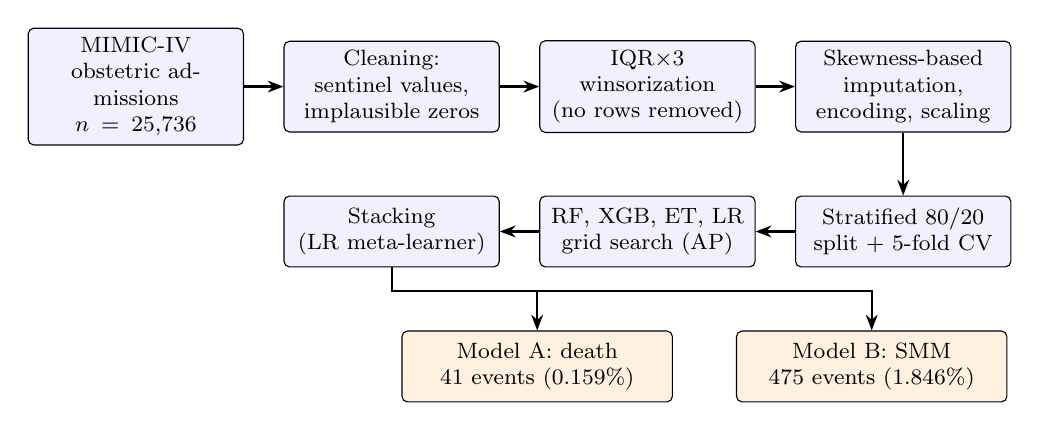
\begin{tikzpicture}[
  node distance=4mm and 5mm,
  box/.style={rectangle,draw,rounded corners=2pt,align=center,font=\footnotesize,
              minimum height=9mm,text width=2.5cm,fill=blue!6},
  outbox/.style={rectangle,draw,rounded corners=2pt,align=center,font=\footnotesize,
              minimum height=9mm,text width=3.2cm,fill=orange!12},
  arr/.style={-{Stealth[length=2mm]},thick}]
\node[box] (a) {MIMIC-IV\\obstetric admissions\\$n=25{,}736$};
\node[box,right=of a] (b) {Cleaning:\\sentinel values,\\implausible zeros};
\node[box,right=of b] (c) {IQR$\times$3\\winsorization\\(no rows removed)};
\node[box,right=of c] (d) {Skewness-based\\imputation,\\encoding, scaling};
\node[box,below=8mm of d] (e) {Stratified 80/20\\split + 5-fold CV};
\node[box,left=of e] (f) {RF, XGB, ET, LR\\grid search (AP)};
\node[box,left=of f] (g) {Stacking\\(LR meta-learner)};
\node[outbox,below=8mm of f,xshift=-14mm] (h) {Model A: death\\41 events (0.159\%)};
\node[outbox,right=8mm of h] (i) {Model B: SMM\\475 events (1.846\%)};
\draw[arr] (a)--(b); \draw[arr] (b)--(c); \draw[arr] (c)--(d);
\draw[arr] (d)--(e); \draw[arr] (e)--(f); \draw[arr] (f)--(g);
\draw[arr] (g.south)--++(0,-3mm)-|(h.north);
\draw[arr] (g.south)--++(0,-3mm)-|(i.north);
\end{tikzpicture}
\caption{Overview of the pipeline. The same cleaning, preprocessing and learning
steps are applied to both outcomes.}\label{fig:pipeline}
\end{figure}

\subsection{Outcome definitions}
\textbf{Model A (mortality).} The outcome is 1 if a hospital death time was
recorded during the index admission or in any later admission of the same patient,
and 0 otherwise. This yielded 41 events among 25{,}736 admissions (0.159\%).

\textbf{Model B (SMM).} An admission is SMM-positive if it carries at least one
ICD-10-CM diagnosis or ICD-10-PCS procedure code matching any of the 20 currently
active CDC/HRSA FAD-2023 indicators~\cite{CDC2023SMM,HRSA2023FAD,Nebraska2024SMM}
(the former indicator on blood-product transfusion, retired by HRSA in 2023, is
excluded). The indicators are grouped into seven clinical categories (cardiac,
renal, respiratory, hemorrhage, sepsis, other obstetric, other medical). There were
475 SMM-positive admissions (1.846\%); among the 8{,}857 delivery hospitalizations,
252 were positive (2.845\%, i.e., 284.5 per 10{,}000), above the published
reference range of 58--88 per 10{,}000 deliveries~\cite{Nebraska2024SMM}.
The higher rate is expected, as MIMIC-IV is a tertiary referral center and the
expanded denominator also includes non-delivery admissions.
The most frequent indicators were acute renal failure (180 admissions), shock (72),
ARDS (66), sepsis (62), and disseminated intravascular coagulation (61); 23.4\% of
positive admissions met indicators from more than one clinical category.

\subsection{Predictors and preprocessing}
Candidate predictors comprised administrative variables (age at admission,
ethnicity group, insurance, language group, admission type, admission location,
ICU stay and ICU stay count) and the earliest available value of 27 chart/laboratory
variables (vital signs, Glasgow Coma Scale components, hematology and chemistry).
For the 13 laboratory variables, values were also taken from hospital-wide
laboratory events (not only from ICU chart events), which matters here
because most deaths occurred outside the ICU. Preprocessing steps were:

\begin{enumerate}[leftmargin=*,labelsep=5.8mm]
\item \textbf{Sentinel values and implausible zeros.} The placeholder 999{,}999 and
      physiologically impossible zeros were set to missing.
\item \textbf{Outlier handling by winsorization.} For each continuous variable,
      values beyond $Q_1 - 3\,\mathrm{IQR}$ or $Q_3 + 3\,\mathrm{IQR}$ were clipped
      to the nearest bound (with clinical lower bounds), so that no admission is
      deleted. Ordinal scales and variables with $\mathrm{IQR}=0$ were not clipped.
      Our first implementation deleted rows with out-of-bound values, as in our
      previous neonatal pipeline; an audit showed that this removed 8 of 41 deaths
      (19.5\%) in Model~A and 184 of 475 SMM cases (38.7\%) in Model~B, so it was
      replaced by winsorization.
\item \textbf{Imputation.} Median for variables with $|\text{skewness}|>1$,
      mode otherwise.
\item \textbf{Encoding and scaling.} One-hot encoding of the five categorical
      groups; \texttt{RobustScaler} for variables with $|\text{skewness}|>1$ and
      \texttt{MinMaxScaler} otherwise. Near-constant ICU-monitoring variables
      (motor GCS and Richmond Agitation--Sedation Scale; the most common value
      covered more than 99\% of rows) were dropped from Model~A.
\end{enumerate}

\textbf{Diagnosis-group indicators and leakage control.} ICD diagnosis codes in the
cohort (4{,}116 distinct codes for Model~A) were aggregated into 26 binary diagnostic
group indicators (\texttt{gdg\_m01}--\texttt{gdg\_m26}) by clinical classification, performed by a panel of four clinical experts (an obstetrician--gynecologist with experience in maternal--fetal medicine, an intensivist with experience in obstetric patients, an internal medicine specialist and an infectious disease specialist) following a structured four-step procedure.
First, all ICD codes in the cohort were tabulated by number and percentage of admissions, and this frequency table
was the panel's working document. Second, codes frequent enough to identify a well-defined clinical
entity were kept as individual groups. Third, less frequent codes were grouped by the experts according to,
in order of priority, a shared pathophysiological mechanism, the affected organ system, and similar
prognostic relevance; no code was assigned to more than one group, and disagreements were settled by discussion
until consensus. Fourth, the complete set was reviewed in a plenary session for clinical coherence, absence of
overlap between groups and sufficient representation in the cohort, and groups that failed these criteria were revised or merged.
Codes that could not be assigned to a clinically interpretable group were reserved for a residual clustering step.
Two further indicators reserved for residual clustering were constant and removed.
Because these indicators are derived from the same coded diagnoses that
define SMM, they were \emph{excluded} from Model~B; likewise the seven per-category
SMM counts, the multiclass label, and the delivery-hospitalization flag were not
used as predictors (the latter is kept only to define the evaluation subset).
Model~A retained the 26 indicators, giving 89 predictors; Model~B used 65 predictors.
This difference in the predictor sets is considered in Section~\ref{sec:discussion}.

Table~\ref{tab:gdg} lists the 26 diagnostic groups. Of the 4{,}116 distinct ICD codes
observed in the cohort (2{,}192 ICD-10 and 1{,}924 ICD-9), 4{,}010 were assigned to one
of the 26 groups and 106 were excluded from grouping; twelve groups are obstetric and
fourteen cover non-obstetric conditions. A k-means step intended to cluster residual,
unassigned codes found no residual codes, so the two reserved cluster indicators were
constant and removed.

\begin{table}[H]
\caption{Diagnostic groups used as binary indicators in Model~A: description, whether the
group is obstetric, and number of distinct ICD codes assigned.\label{tab:gdg}}
\small
\begin{tabularx}{\textwidth}{llcc}
\toprule
\textbf{Indicator} & \textbf{Group} & \textbf{Obstetric} & \textbf{ICD codes}\\
\midrule
gdg\_m01 & Labor and delivery complications & Yes & 225 \\
gdg\_m02 & Pre-existing condition complicating pregnancy & Yes & 167 \\
gdg\_m03 & Hypertensive disorders of pregnancy & Yes & 95 \\
gdg\_m04 & Other pregnancy-related maternal disorders & Yes & 83 \\
gdg\_m05 & Fetal complications / multiple gestation & Yes & 156 \\
gdg\_m06 & Other puerperal complications & Yes & 27 \\
gdg\_m07 & Placental / amniotic fluid disorders & Yes & 43 \\
gdg\_m08 & Hemorrhage (antepartum/postpartum) & Yes & 57 \\
gdg\_m09 & Infection (obstetric/puerperal) & Yes & 117 \\
gdg\_m10 & Preterm labor / premature rupture of membranes & Yes & 35 \\
gdg\_m11 & Abortion / ectopic or molar pregnancy & Yes & 103 \\
gdg\_m12 & Venous / thromboembolic disorders & Yes & 50 \\
gdg\_m13 & Neoplasms & No & 95 \\
gdg\_m14 & Digestive diseases & No & 248 \\
gdg\_m15 & Endocrine / metabolic / nutritional disorders & No & 197 \\
gdg\_m16 & Cardiovascular diseases & No & 231 \\
gdg\_m17 & Nervous system disorders & No & 147 \\
gdg\_m18 & Blood / immune system diseases & No & 107 \\
gdg\_m19 & Genitourinary diseases (non-obstetric) & No & 175 \\
gdg\_m20 & Respiratory diseases & No & 106 \\
gdg\_m21 & Administrative factors / contact with health services & No & 306 \\
gdg\_m22 & Symptoms, signs and ill-defined findings & No & 208 \\
gdg\_m23 & Infectious and parasitic diseases & No & 147 \\
gdg\_m24 & Injury, poisoning and external causes & No & 355 \\
gdg\_m25 & Other minor comorbidities & No & 332 \\
gdg\_m26 & Mental and behavioral disorders & No & 198 \\
\bottomrule
\end{tabularx}
\end{table}

\subsection{Correlation analysis}
Collinearity was reviewed in two passes: a heatmap of all continuous clinical variables
and a focused pass over the binary diagnostic indicators, using $|r|\geq 0.70$ as the
threshold for a strongly correlated pair. Because the tree-based learners evaluate
features independently at each split and the logistic regression is L2-regularized, we
retained all correlated variables, since dropping one member of a physiologically
paired measurement would discard independently monitored signal without a modelling
benefit.

\subsection{Learning algorithms and evaluation}
We trained Random Forest (RF), XGBoost (XGB), Extra Trees (ET) and L2-regularized
Logistic Regression (LR) on an 80/20 stratified split (random seed 42):
20{,}588 training and 5{,}148 test admissions, with 33 and 8 deaths in Model~A and
380 and 95 SMM cases in Model~B. Imbalance was handled through class weighting
(\texttt{balanced} or \texttt{balanced\_subsample}; XGB \texttt{scale\_pos\_weight}
of 622.9 in A and 53.2 in B). Hyperparameters were tuned with grid search using
stratified five-fold cross-validation on the training set with \emph{average
precision} as the criterion; grids were deliberately small for Model~A. The tuned
learners were combined into a stacked ensemble~\cite{Wolpert1992Stacking} with a
class-weighted L2 logistic-regression meta-learner whose inputs were generated by
the same five-fold stratified scheme. Implementation used scikit-learn,
XGBoost and imbalanced-learn~\cite{Pedregosa2011sklearn,Chen2016XGBoost,Chawla2002SMOTE}
with RF~\cite{Breiman2001RF} and ET~\cite{Geurts2006ExtraTrees} base models. The selected hyperparameters of every learner are listed in Table~\ref{tab:hyper}.

\begin{table}[H]
\caption{Selected hyperparameters (grid search, five-fold stratified cross-validation on the training split, criterion: average precision).
Both forests used \texttt{max\_features} = sqrt; class weights were \texttt{balanced\_subsample} for RF and \texttt{balanced} for ET and LR.\label{tab:hyper}}
\small
\begin{tabularx}{\textwidth}{lXX}
\toprule
\textbf{Model} & \textbf{Model A (mortality)} & \textbf{Model B (SMM)}\\
\midrule
Random Forest & 400 trees; max depth 20; min split 2; min leaf 2 & 300 trees; max depth 20; min split 10; min leaf 4\\
XGBoost & 400 trees; max depth 5; learning rate 0.1; subsample 0.8; column sample 1.0; positive-class weight 622.9 & 600 trees; max depth 3; learning rate 0.01; subsample 0.8; column sample 0.8; positive-class weight 53.2\\
Extra Trees & 400 trees; max depth none; min split 2; min leaf 1 & 500 trees; max depth 20; min split 10; min leaf 2\\
Logistic Regression & L2; $C=0.01$; solver saga; 3{,}000 iterations & L2; $C=5$; solver lbfgs; 3{,}000 iterations\\
Stacking (meta-learner) & \multicolumn{2}{p{0.6\textwidth}}{L2 logistic regression; $C=0.1$; solver lbfgs; 5{,}000 iterations; balanced class weights; five-fold out-of-fold inputs}\\
\bottomrule
\end{tabularx}
\end{table}


ROC and precision--recall (PR) curves~\cite{Fawcett2006ROC,Saito2015PR} and the AUC and AP were computed from predicted
probabilities of the positive class, while the classification report and confusion
matrix used the default 0.5 decision threshold. Since only 8 deaths fall in the
Model~A test set, the main evidence for Model~A is stratified five-fold
cross-validation over all 25{,}736 admissions, reported as mean $\pm$ standard
deviation for AUC, AP, recall, F1 and balanced accuracy~\cite{Arlot2010CV}. Formal sample-size criteria for prediction models depend on the number of candidate predictors, the outcome prevalence and the expected performance~\cite{Riley2020SampleSize}; with 41 events and 89 candidate predictors (about 0.5 events per predictor), Model~A is unlikely to meet them, which is a further reason to treat its results as exploratory. The
cross-validation re-fits the already tuned configurations on the full data set; its
estimates are therefore slightly optimistic, as the hyperparameters were selected on
the training split. As a sensitivity analysis, SMOTE (sampling strategy 0.2,
$k=5$) was placed inside each training fold of a pipeline to avoid leakage into the
validation folds. For Model~B, the stacked ensemble was additionally evaluated on
the delivery-hospitalization subset of the test set, without re-training.
The study follows the TRIPOD+AI reporting guidance where applicable~\cite{Collins2024TRIPODAI}
(the completed checklist is provided as Supplementary Material).

\subsection{Additional analyses}\label{sec:additional}
Six further analyses complement the main evaluation.
(i)~\emph{Cross-validation for Model~B}: the same stratified five-fold protocol applied to
Model~A was applied to Model~B, so that both outcomes are assessed with the same primary
evidence; a SMOTE variant was run in the same way.
(ii)~\emph{Model~A without diagnostic groups}: Model~A was re-evaluated by cross-validation
after removing the 26 diagnostic-group indicators, keeping the tuned hyperparameters, so
that its predictor set matches that of Model~B.
(iii)~\emph{Calibration and risk stratification}: out-of-fold probabilities of the stacked
ensemble over the full cohort were used to compute the Brier score~\cite{Brier1950} and its skill relative to
a model that predicts the prevalence, the ratio between mean predicted probability and
observed prevalence, a reliability curve with quantile bins~\cite{VanCalster2019Calibration,Guo2017Calibration}, and ``flag the top $x$\%''
tables giving recall, positive predictive value and lift. Risk bands were defined from the
model's own probability percentiles (low: below the 80th percentile; moderate: 80th to 95th;
high: top 5\%), because fixed cut-offs are not meaningful at these prevalences, and
bootstrap 95\% confidence intervals (500 resamples) were computed.
(iv)~\emph{Explainability}: TreeSHAP values~\cite{Lundberg2017SHAP,Lundberg2020TreeSHAP} of the fitted XGBoost base learner were computed on
the Model~B test set.
(v)~\emph{Subgroup audit}: the hold-out performance of the Model~B stacked ensemble was
described by ethnicity group, insurance, age quartile, ICU stay and delivery versus
non-delivery admission, reporting AUC with bootstrap confidence intervals only for
subgroups with at least 10 positive and 10 negative admissions. Auditing performance by subgroup responds to documented concerns that algorithms can reproduce or amplify inequities in health care~\cite{Obermeyer2019Bias,Rajkomar2018Fairness}.
(vi)~\emph{Recalibration}: because class weighting inflates the predicted probabilities, Platt scaling (a logistic regression on the logit of the stacked probability) and isotonic regression were fitted to the out-of-fold probabilities inside repeated (20 times) five-fold cross-validation, without retraining the models, and evaluated with the Brier score and its skill, the ratio of mean predicted probability to prevalence, the expected calibration error (ECE, ten quantile bins), the calibration slope and intercept, AUC and AP.

%--------------------------------------------------------------------
\section{Results}\label{sec:results}
%--------------------------------------------------------------------
\subsection{Cohorts and outcomes}
Table~\ref{tab:cohort} compares the two prediction tasks. Model~B has 11.6 times
more events than Model~A and 95 rather than 8 positives in the test set.

\begin{table}[H]
\caption{Comparison of the two prediction tasks (same 25{,}736 admissions).\label{tab:cohort}}
\newcolumntype{C}{>{\centering\arraybackslash}X}
\begin{tabularx}{\textwidth}{lCC}
\toprule
 & \textbf{Model A (mortality)} & \textbf{Model B (SMM)}\\
\midrule
Positive admissions & 41 (0.159\%) & 475 (1.846\%)\\
Positives in training / test split & 33 / 8 & 380 / 95\\
Predictors & 89 (incl.\ 26 diagnosis groups) & 65 (no diagnosis groups)\\
Weight for the positive class (XGBoost) & 622.9 & 53.2\\
Positives retained after outlier handling & 41 of 41 & 475 of 475\\
\bottomrule
\end{tabularx}
\end{table}

\subsection{Descriptive analysis of severe maternal morbidity}
All 20 CDC/HRSA indicators were observed at least once. Table~\ref{tab:smm} lists the
number of admissions per indicator. Renal indicators were the most frequent category
(180 admissions with at least one renal indicator), followed by hemorrhage (131),
respiratory (89), other medical (77), sepsis (62), cardiac (61) and other obstetric
(56) indicators. When each SMM admission was assigned to the category with the most
indicators, the primary categories were renal (132), hemorrhage (115), other medical
(71), cardiac (52), other obstetric (38), respiratory (36) and sepsis (31).
Most SMM admissions involved a single clinical category (364 of 475, 76.6\%), whereas 64
involved two, 27 three, 17 four and 3 five categories (111 admissions, 23.4\%, with more than
one category). The most frequent pairs were respiratory with hemorrhage (42 admissions), renal with
hemorrhage (37), renal with respiratory (28), cardiac with respiratory (26) and
hemorrhage with sepsis (20) (Figure~\ref{fig:smmdesc}). The SMM rate was 184.6 per 10{,}000
admissions in the expanded cohort and 284.5 per 10{,}000 in delivery hospitalizations, against
a published range of 58--88 per 10{,}000 deliveries.

\begin{table}[H]
\caption{Admissions per CDC/HRSA SMM indicator, grouped by clinical category
(an admission may contain several indicators).\label{tab:smm}}
\small
\begin{tabularx}{\textwidth}{llc}
\toprule
\textbf{Category} & \textbf{Indicator} & \textbf{Admissions}\\
\midrule
\multirow{6}{*}{Cardiac} & Pulmonary edema / acute heart failure & 45\\
 & Conversion of cardiac rhythm & 8\\
 & Acute myocardial infarction & 7\\
 & Cardiac arrest / ventricular fibrillation & 7\\
 & Aneurysm & 5\\
 & Heart failure / arrest during surgery or procedure & 1\\
\midrule
\multirow{3}{*}{Hemorrhage} & Shock & 72\\
 & Disseminated intravascular coagulation & 61\\
 & Hysterectomy & 41\\
\midrule
\multirow{2}{*}{Other medical} & Puerperal cerebrovascular disorders & 55\\
 & Sickle cell disease with crisis & 23\\
\midrule
\multirow{4}{*}{Other obstetric} & Air and thrombotic embolism & 33\\
 & Eclampsia & 16\\
 & Amniotic fluid embolism & 4\\
 & Severe anesthesia complications & 4\\
\midrule
Renal & Acute renal failure & 180\\
\midrule
\multirow{3}{*}{Respiratory} & Acute respiratory distress syndrome & 66\\
 & Ventilation & 51\\
 & Temporary tracheostomy & 1\\
\midrule
Sepsis & Sepsis & 62\\
\bottomrule
\end{tabularx}
\end{table}
\unskip
\begin{figure}[H]
\centering
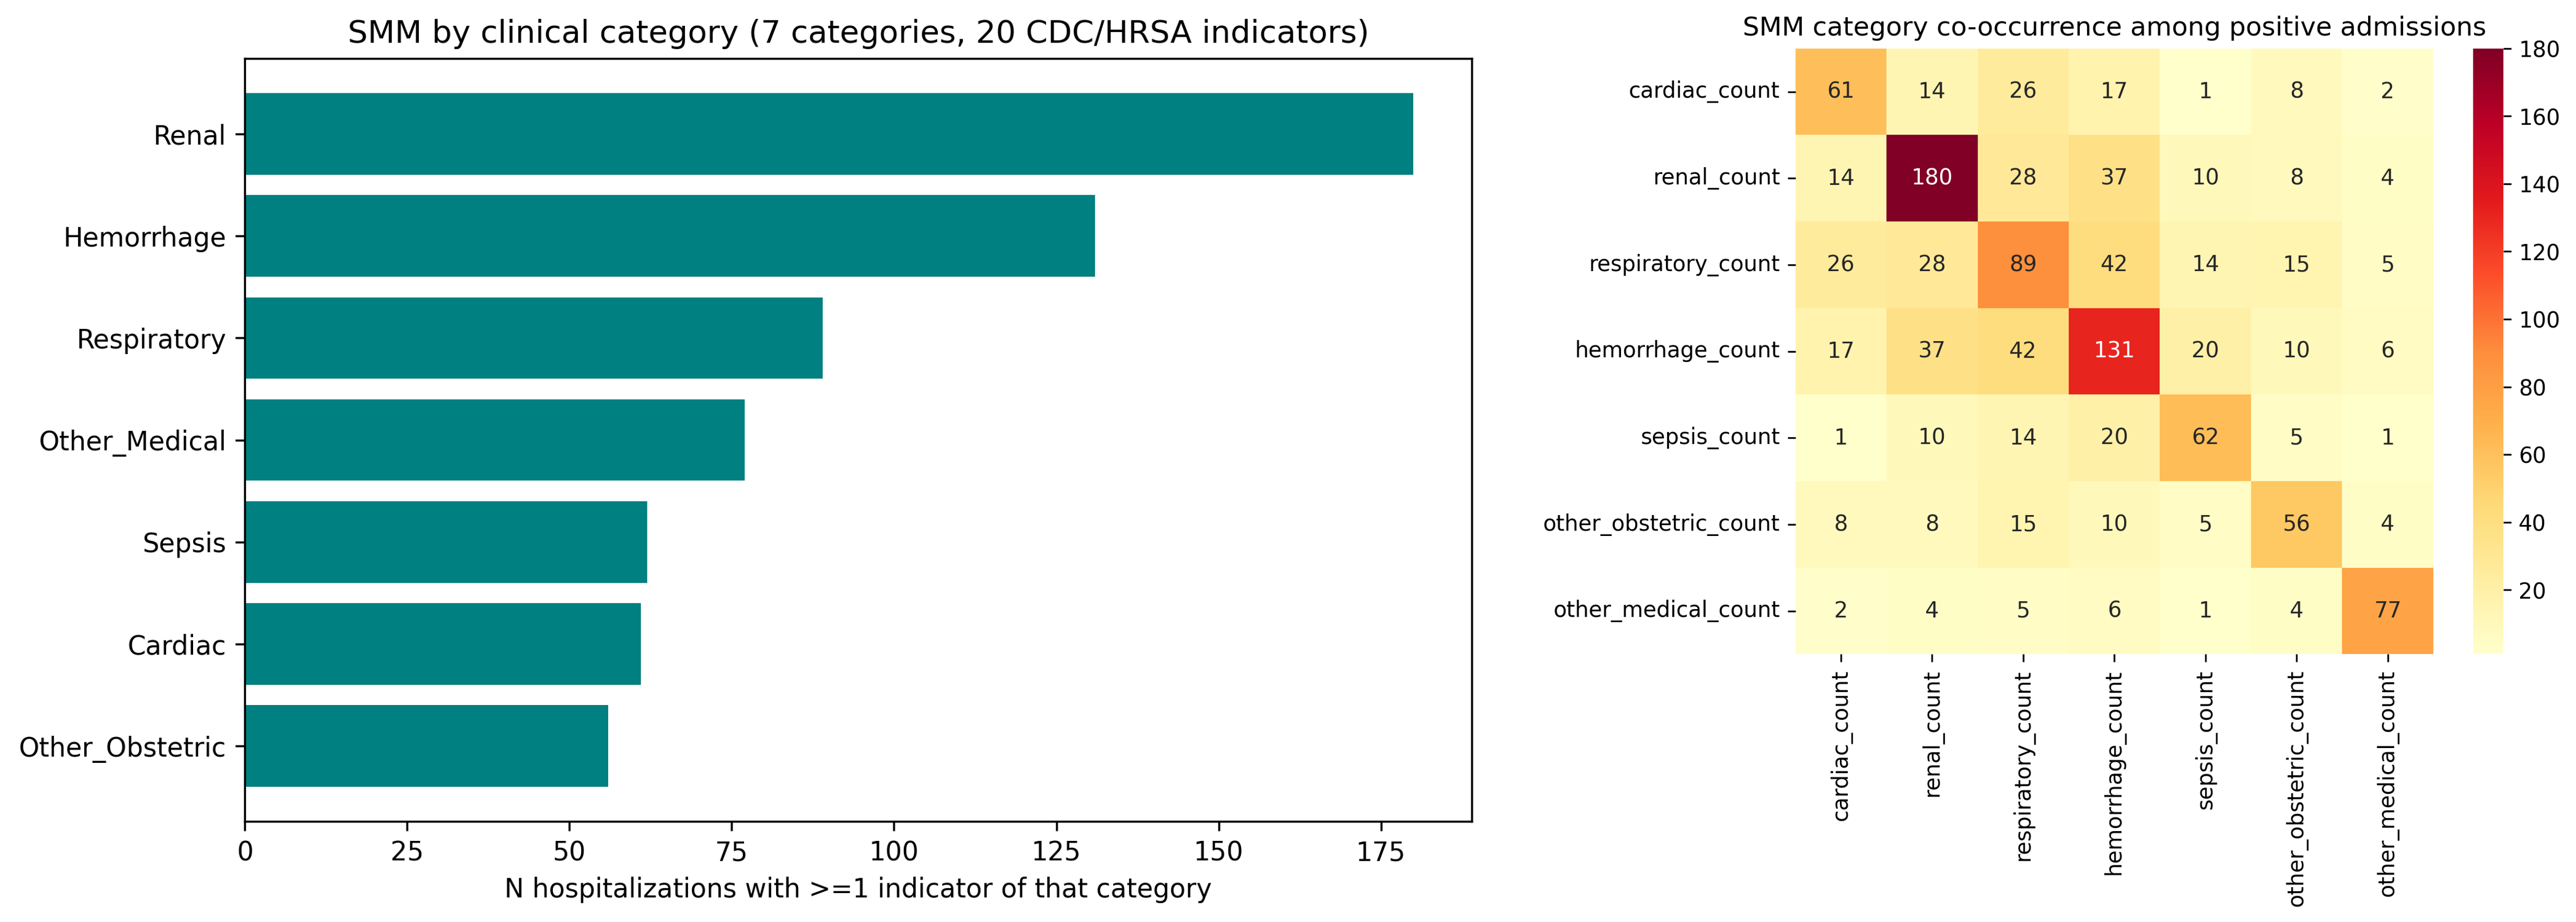
\includegraphics[width=\textwidth]{fig_smm_descriptive.png}
\caption{SMM admissions by clinical category (left) and co-occurrence of categories among
SMM admissions (right; the diagonal gives the number of admissions per category).}\label{fig:smmdesc}
\end{figure}

\subsection{Correlation structure of the predictors}
Ten pairs of clinical variables had $|r|\geq 0.70$ (Table~\ref{tab:corr}), all physiologically
expected: ICU stay and ICU stay count, the three blood-pressure measures, the Glasgow Coma
Scale components with the Richmond Agitation--Sedation Scale, and hemoglobin with hematocrit.
Following the policy in Section~\ref{sec:methods}, no variable was removed for collinearity.
Motor GCS and the Richmond scale were dropped from Model~A for near-zero variance (most common
value in more than 99\% of rows), and were retained in Model~B.

\begin{table}[H]
\caption{Pairs of clinical variables with $|r|\geq 0.70$ (identical in both models).\label{tab:corr}}
\begin{tabularx}{\textwidth}{llc}
\toprule
\textbf{Variable 1} & \textbf{Variable 2} & \textbf{$r$}\\
\midrule
ICU stay & ICU stay count & 0.958\\
Mean blood pressure & Diastolic blood pressure & 0.907\\
GCS eye opening & GCS verbal response & 0.891\\
GCS eye opening & GCS motor response & 0.882\\
Hemoglobin & Hematocrit & 0.839\\
Mean blood pressure & Systolic blood pressure & 0.833\\
GCS eye opening & Richmond Agitation--Sedation Scale & 0.783\\
GCS verbal response & GCS motor response & 0.773\\
GCS verbal response & Richmond Agitation--Sedation Scale & 0.754\\
GCS motor response & Richmond Agitation--Sedation Scale & 0.747\\
\bottomrule
\end{tabularx}
\end{table}

\subsection{Model A: mortality}
Table~\ref{tab:cvA} and Figure~\ref{fig:cvA} show the cross-validated results.
The stacked ensemble had the highest AUC (0.857 $\pm$ 0.069) and the highest
balanced accuracy and recall (0.780 and 0.731), but its F1 score was only
0.014, and its AP (0.156 $\pm$ 0.096) was lower than that of XGB and ET
(0.165 and 0.190), although within one standard deviation of both, and far below any clinically useful level in absolute terms,
although it is roughly one hundred times the prevalence of 0.0016. Fold-to-fold
variability was large (the standard deviation of AP reached 0.119 for XGB and 0.096 for
the stacked ensemble) and RF produced no positive predictions at the default
threshold (recall 0). LR had the lowest AUC and AP (0.758 and 0.049). On the
hold-out test set (8 deaths), AUC values ranged from 0.786 (RF) to 0.858 (XGB and ET), with
the stacked ensemble at 0.844 and an AP of 0.148, whereas XGB had the highest AP (0.278) (Table~\ref{tab:holdout}). The
confusion matrix of the stacked ensemble contained 7 true positives, 1 false negative, 799 false positives
and 4{,}341 true negatives (recall 0.88, precision 0.009); these point estimates rest on
eight patients and must be read as illustrative only.

\begin{table}[H]
\caption{Model~A: stratified five-fold cross-validation (mean $\pm$ SD) on all
25{,}736 admissions (41 deaths).\label{tab:cvA}}
\scriptsize
\setlength{\tabcolsep}{3pt}
\begin{tabularx}{\textwidth}{lCCCCC}
\toprule
\textbf{Model} & \textbf{AUC} & \textbf{AP} & \textbf{Recall} & \textbf{F1} & \textbf{Bal.\ acc.}\\
\midrule
Random Forest & 0.809 $\pm$ 0.042 & 0.115 $\pm$ 0.091 & 0.000 $\pm$ 0.000 & 0.000 $\pm$ 0.000 & 0.500 $\pm$ 0.000\\
XGBoost & 0.817 $\pm$ 0.045 & 0.165 $\pm$ 0.119 & 0.117 $\pm$ 0.145 & \textbf{0.137 $\pm$ 0.172} & 0.558 $\pm$ 0.073\\
Extra Trees & 0.831 $\pm$ 0.051 & 0.190 $\pm$ 0.086 & 0.050 $\pm$ 0.061 & 0.089 $\pm$ 0.109 & 0.525 $\pm$ 0.031\\
Logistic Regression & 0.758 $\pm$ 0.065 & 0.049 $\pm$ 0.058 & 0.631 $\pm$ 0.213 & 0.012 $\pm$ 0.004 & 0.735 $\pm$ 0.101\\
Stacking & 0.857 $\pm$ 0.069 & 0.156 $\pm$ 0.096 & \textbf{0.731 $\pm$ 0.124} & 0.014 $\pm$ 0.002 & \textbf{0.780 $\pm$ 0.058}\\
\bottomrule
\end{tabularx}
\end{table}
\unskip
\begin{figure}[H]
\centering
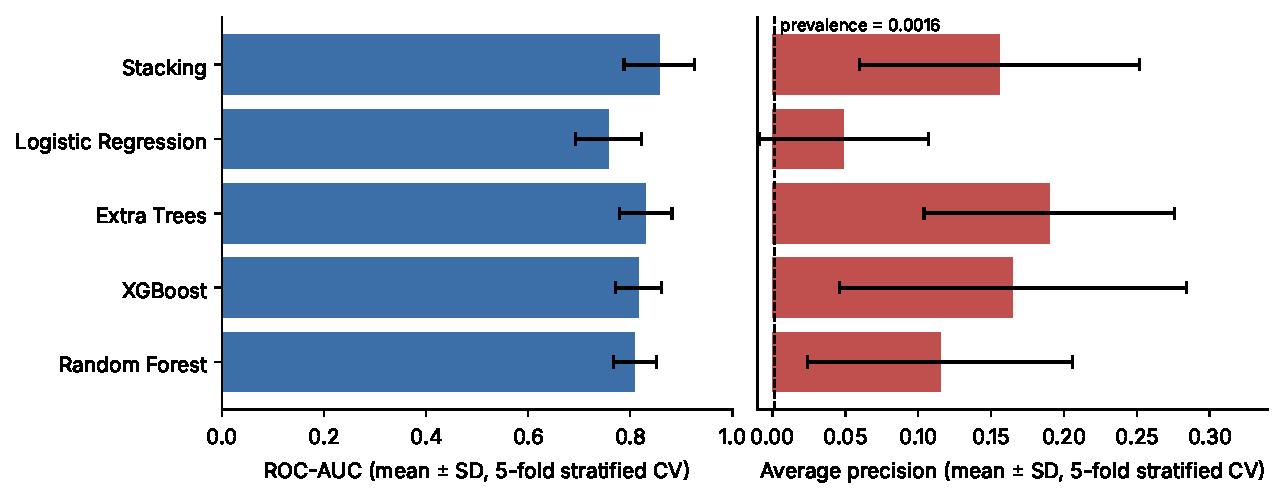
\includegraphics[width=0.85\textwidth]{fig_cv_modelA.pdf}
\caption{Model~A: cross-validated AUC and average precision with standard deviations.
The dashed line marks the outcome prevalence (41/25{,}736).}\label{fig:cvA}
\end{figure}

\subsection{Oversampling sensitivity analysis (Model A)}
Adding SMOTE inside each training fold increased the AUC of all five models
(e.g., stacking 0.857 to 0.870, XGB 0.817 to 0.854, ET 0.831 to 0.848) and the recall of RF, XGB
and ET, but not that of the stacked ensemble (0.731 to 0.142) or LR (0.631 to 0.267).
AP changed little: it rose for stacking (0.156 to 0.168), XGB (0.165 to 0.173), RF (0.115 to 0.128)
and LR (0.049 to 0.052) and fell for ET (0.190 to 0.173)
(Table~\ref{tab:smote}, Figure~\ref{fig:smote}). The changes in AUC and AP are all
smaller than one standard deviation, whereas the recall of the stacked ensemble
dropped markedly. Since oversampling mainly shifts the operating point rather than
adding information, and AP did not improve beyond fold-to-fold noise, class weighting
was kept as the default.

\begin{table}[H]
\caption{Model~A: effect of SMOTE (sampling strategy 0.2) on five-fold
cross-validated AUC, AP and recall (mean values).\label{tab:smote}}
\small
\begin{tabularx}{\textwidth}{lCCCCCC}
\toprule
 & \multicolumn{2}{c}{\textbf{AUC}} & \multicolumn{2}{c}{\textbf{AP}} & \multicolumn{2}{c}{\textbf{Recall}}\\
\cmidrule(lr){2-3}\cmidrule(lr){4-5}\cmidrule(lr){6-7}
\textbf{Model} & Weights & SMOTE & Weights & SMOTE & Weights & SMOTE\\
\midrule
Random Forest & 0.809 & 0.842 & 0.115 & 0.128 & 0.000 & 0.097\\
XGBoost & 0.817 & 0.854 & 0.165 & 0.173 & 0.117 & 0.142\\
Extra Trees & 0.831 & 0.848 & 0.190 & 0.173 & 0.050 & 0.097\\
Logistic Regression & 0.758 & 0.809 & 0.049 & 0.052 & 0.631 & 0.267\\
Stacking & 0.857 & 0.870 & 0.156 & 0.168 & 0.731 & 0.142\\
\bottomrule
\end{tabularx}
\end{table}
\unskip
\begin{figure}[H]
\centering
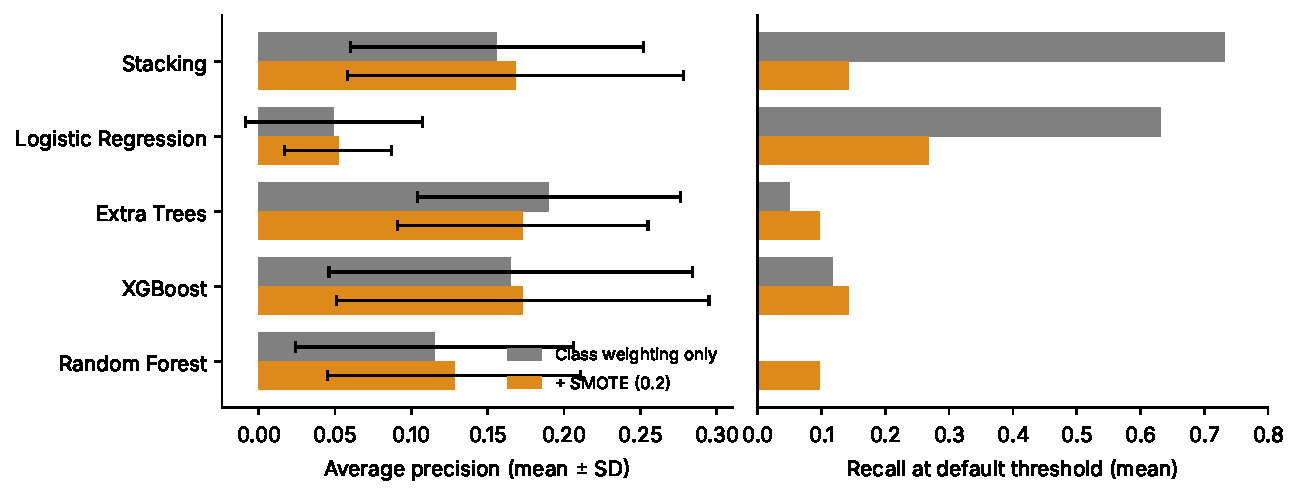
\includegraphics[width=0.95\textwidth]{fig_smote_modelA.pdf}
\caption{Model~A: class weighting versus SMOTE in five-fold cross-validation.}\label{fig:smote}
\end{figure}

\subsection{Model B: severe maternal morbidity}
Model~B showed a better and much more stable behavior. On the hold-out test set
(95 SMM cases), the stacked ensemble was the best model in both AUC (0.913) and
AP (0.384), followed by XGB (AUC 0.909, AP 0.358) and RF (AUC 0.900, AP 0.360)
(Table~\ref{tab:holdout}). The AP of the stacked ensemble is about 21 times the
test prevalence (0.018). At the default threshold its confusion matrix showed 75
true positives, 20 false negatives, 473 false positives and 4{,}580 true negatives
(recall 0.79, precision 0.14). Restricted to the 1{,}802 test admissions that were
delivery hospitalizations (58 SMM cases, 3.219\%), the same model reached a recall
of 0.78, precision of 0.27, F1 of 0.40 for the positive class and an AP of 0.646
(versus 0.384 in the whole test set), with an overall accuracy of 0.93. Figure~\ref{fig:rocpr}
shows the ROC and PR curves of the stacked ensemble for both models.

\begin{table}[H]
\caption{Hold-out test performance (probabilities of the positive class): AUC and
average precision. Model~A test set: 5{,}148 admissions, 8 deaths; Model~B test set:
5{,}148 admissions, 95 SMM cases.\label{tab:holdout}}
\begin{tabularx}{\textwidth}{lCCCC}
\toprule
 & \multicolumn{2}{c}{\textbf{Model A (mortality)}} & \multicolumn{2}{c}{\textbf{Model B (SMM)}}\\
\cmidrule(lr){2-3}\cmidrule(lr){4-5}
\textbf{Model} & AUC & AP & AUC & AP\\
\midrule
Random Forest & 0.786 & 0.065 & 0.900 & 0.360\\
XGBoost & \textbf{0.858} & \textbf{0.278} & 0.909 & 0.358\\
Extra Trees & \textbf{0.858} & 0.161 & 0.900 & 0.315\\
Logistic Regression & 0.854 & 0.031 & 0.889 & 0.339\\
Stacking & 0.844 & 0.148 & \textbf{0.913} & \textbf{0.384}\\
\bottomrule
\end{tabularx}
\end{table}
\unskip
\begin{figure}[H]
\centering
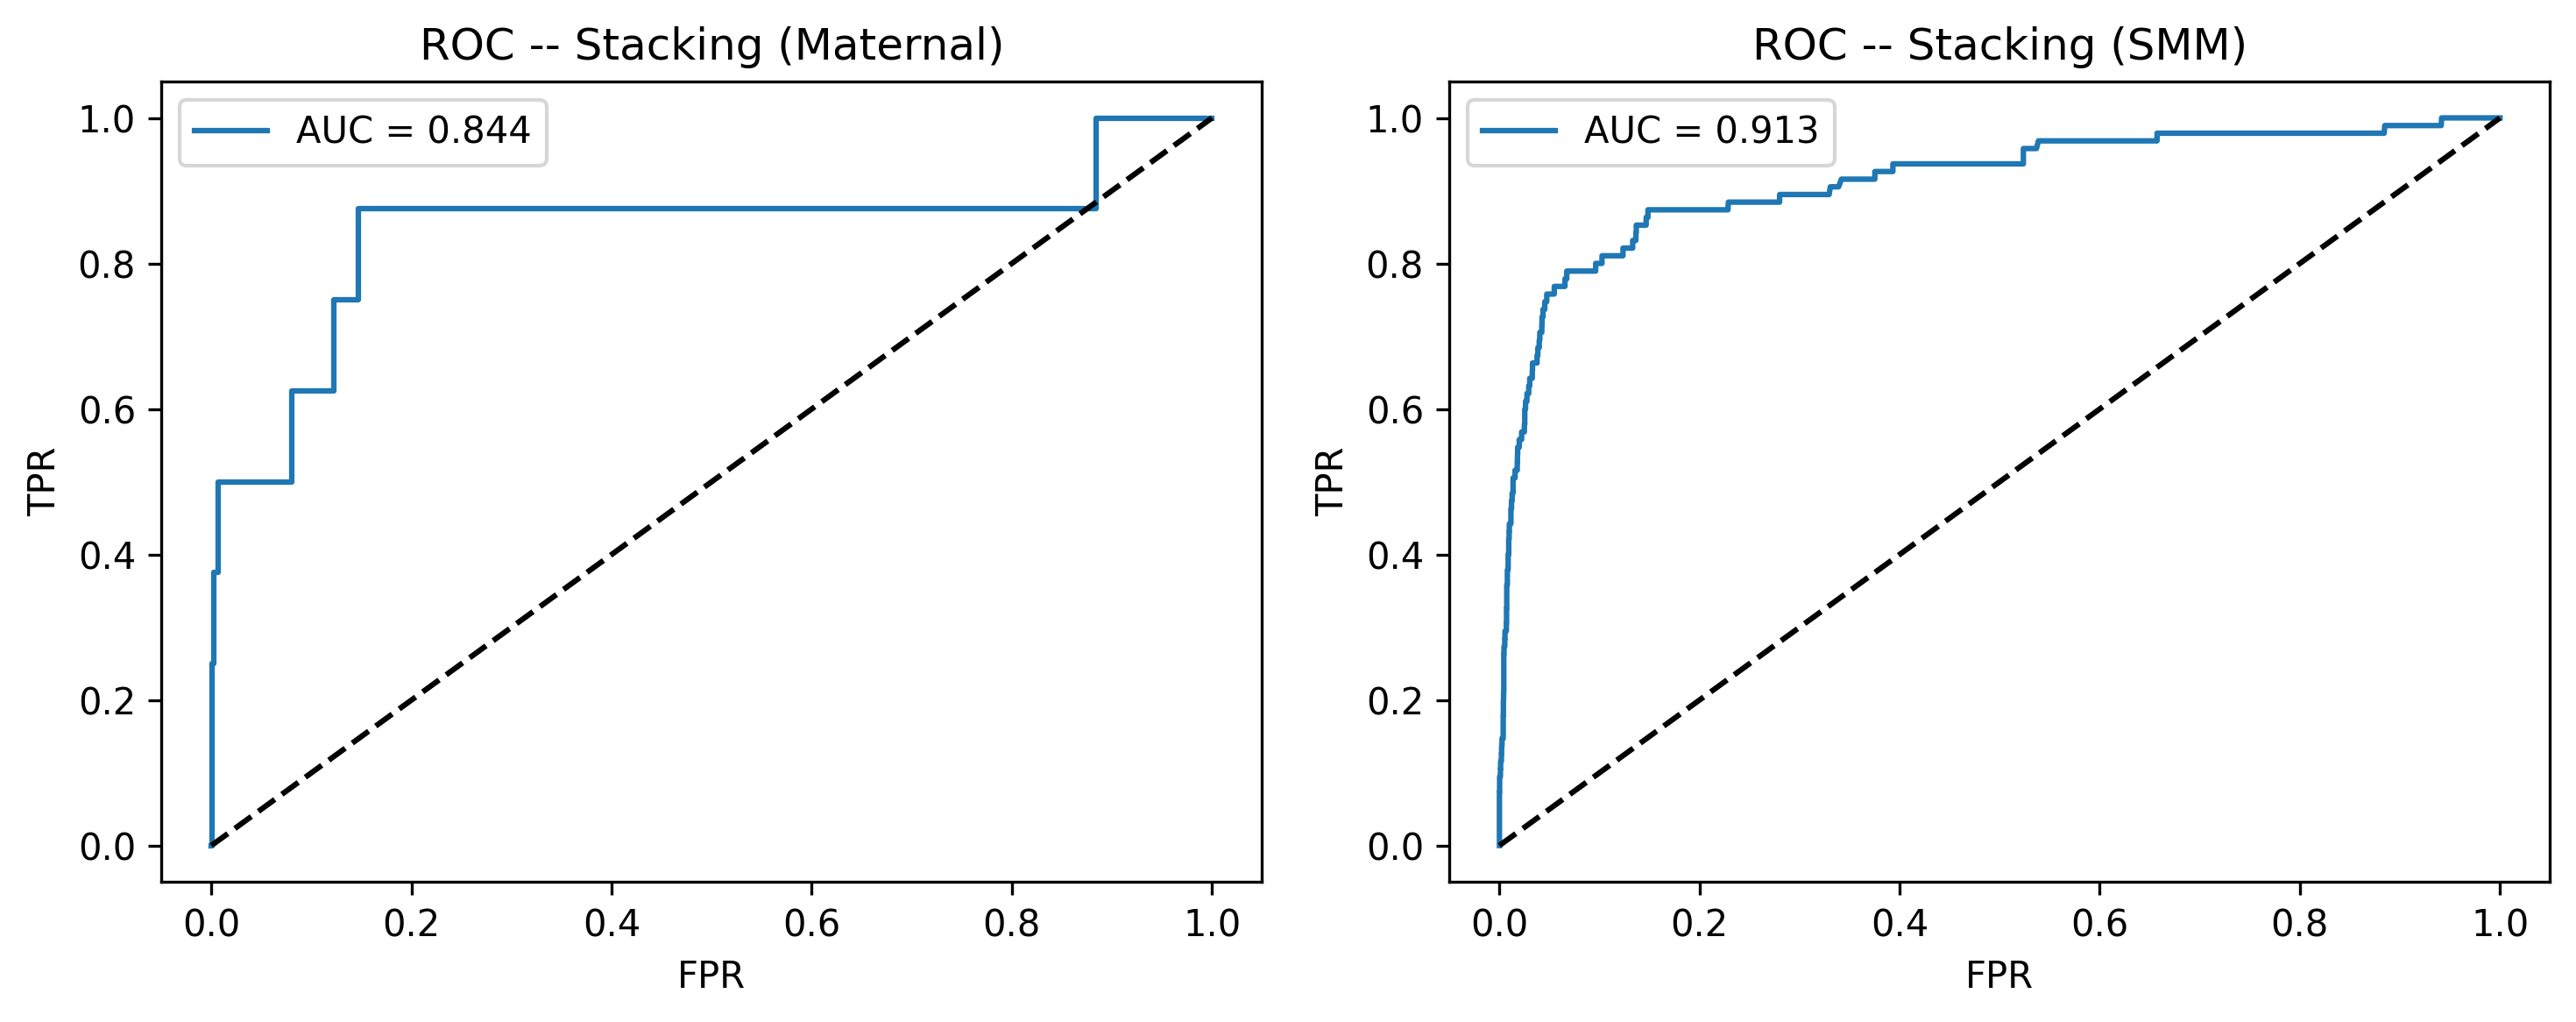
\includegraphics[width=\textwidth]{fig_roc_stacking.png}\\[2mm]
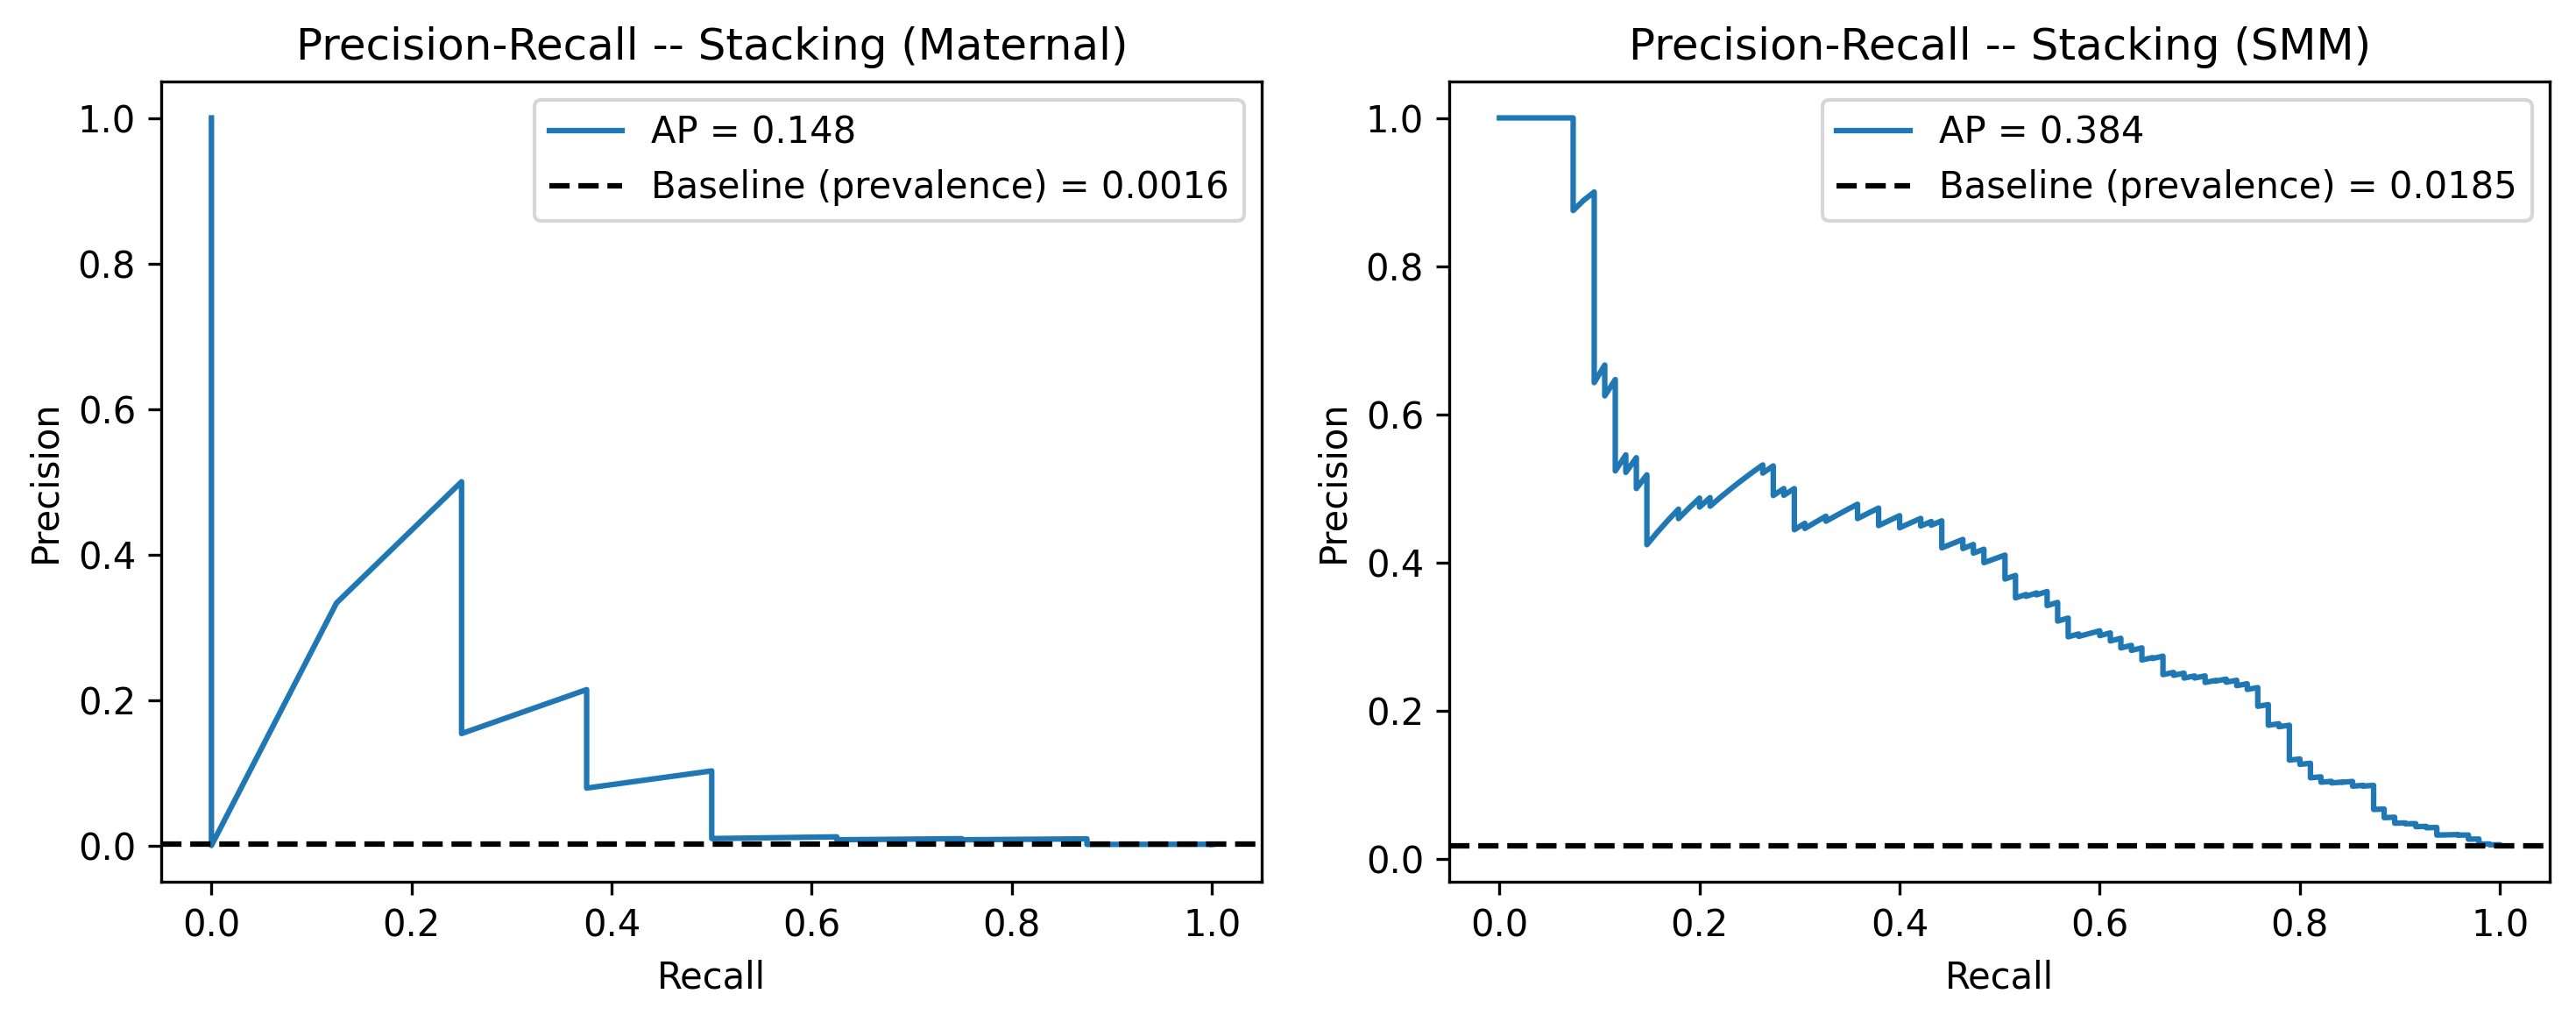
\includegraphics[width=\textwidth]{fig_pr_stacking.png}
\caption{ROC (top) and precision--recall (bottom) curves of the stacked ensemble on
the hold-out set. Left: Model~A; right: Model~B.}\label{fig:rocpr}
\end{figure}

\subsection{Predictor importance}
Figure~\ref{fig:importance} shows the 30 most important predictors of the tuned Random
Forest for each model. For Model~A, age at admission ranked first, followed by
hematocrit, hemoglobin and the diagnosis-group indicators \texttt{gdg\_m13}
and \texttt{gdg\_m03}. For Model~B, the top positions were occupied by laboratory values:
creatinine, glucose, bicarbonate, magnesium, and hemoglobin. Impurity-based
importances are descriptive of the fitted forests and not evidence of causal
effects; moreover, the importance threshold used for feature screening was
computed but not applied, so that all predictors were retained in every model.

\begin{figure}[H]
\centering
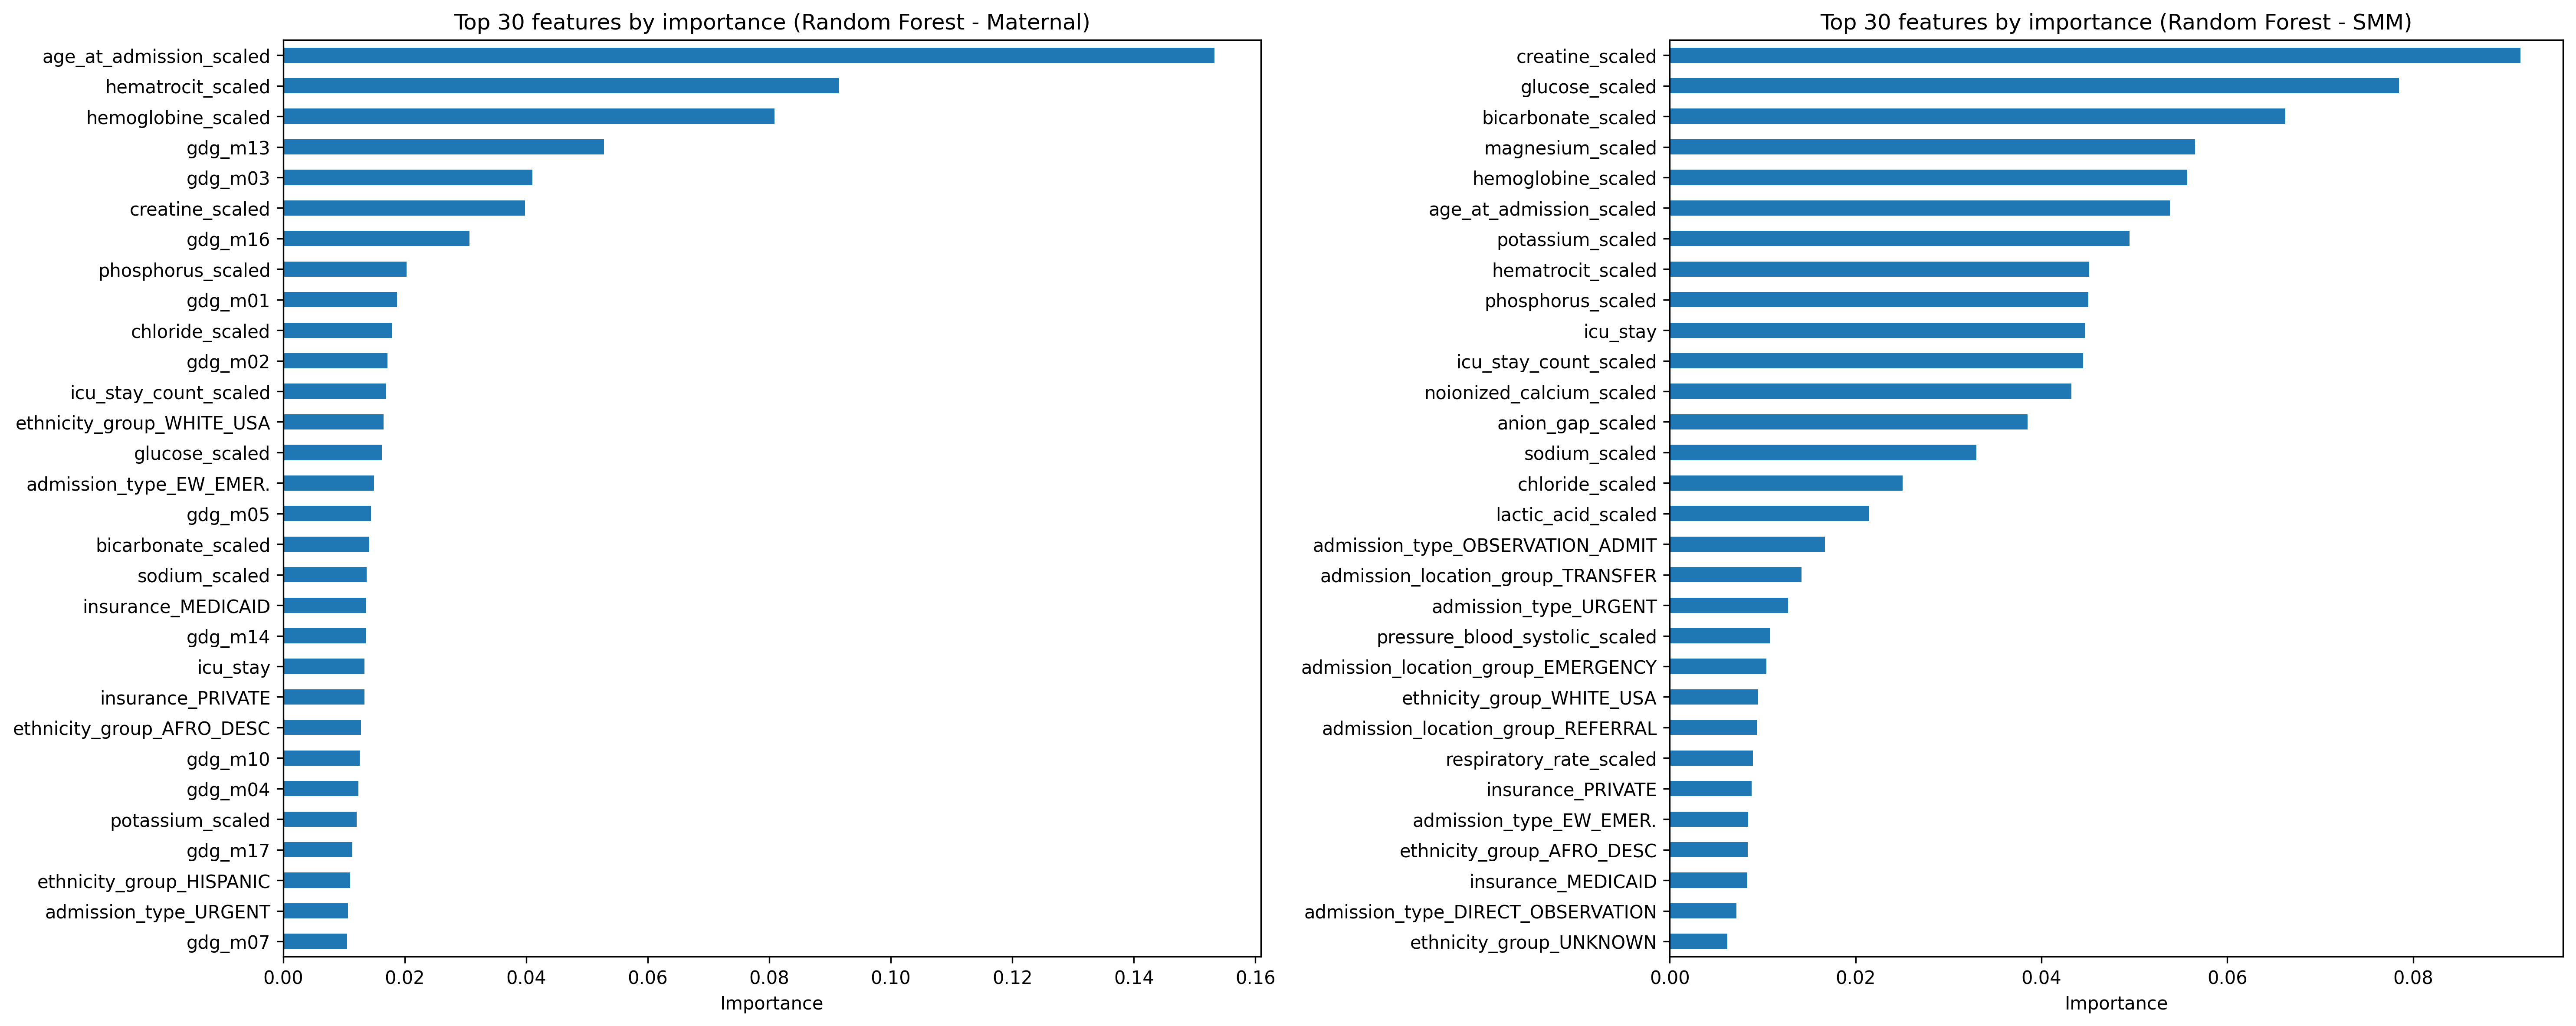
\includegraphics[width=\textwidth]{fig_importance.png}
\caption{Top 30 Random Forest feature importances. Left: Model~A; right: Model~B.}\label{fig:importance}
\end{figure}

\subsection{Additional analyses}
\paragraph{Cross-validation for Model B.}
Over the full cohort (475 SMM cases), the same five-fold protocol gave results that were
consistent with the hold-out evaluation and considerably less dispersed than those of Model~A
(Table~\ref{tab:cvB}, Figure~\ref{fig:cvB}). The stacked ensemble had the highest AUC and AP
(0.904 $\pm$ 0.020 and 0.419 $\pm$ 0.050, about 23 times the prevalence), with XGBoost nearly identical
(0.901 and 0.413); the standard deviations of the AUC across folds were 0.017--0.029, against 0.042--0.069
for Model~A. The stacked ensemble was also the best model on the hold-out set (AUC 0.913, AP 0.384), although the differences among the top models
are smaller than one standard deviation of AP. The operating point at the default threshold differed
markedly between models: the stacked ensemble and XGBoost reached recall of 0.800 and 0.758 at the cost of low
F1 (0.234 and 0.264), whereas Random Forest was more conservative (recall 0.467, F1 0.444).

\begin{table}[H]
\caption{Model~B: stratified five-fold cross-validation (mean $\pm$ SD) on all 25{,}736 admissions
(475 SMM cases).\label{tab:cvB}}
\small
\begin{tabularx}{\textwidth}{lCCCC}
\toprule
\textbf{Model} & \textbf{AUC} & \textbf{AP} & \textbf{Recall} & \textbf{F1}\\
\midrule
Random Forest & 0.890 $\pm$ 0.028 & 0.368 $\pm$ 0.037 & 0.467 $\pm$ 0.034 & 0.444 $\pm$ 0.032\\
XGBoost & 0.901 $\pm$ 0.017 & 0.413 $\pm$ 0.038 & 0.758 $\pm$ 0.040 & 0.264 $\pm$ 0.011\\
Extra Trees & 0.885 $\pm$ 0.023 & 0.359 $\pm$ 0.042 & 0.560 $\pm$ 0.041 & 0.362 $\pm$ 0.035\\
Logistic Regression & 0.876 $\pm$ 0.029 & 0.342 $\pm$ 0.048 & 0.749 $\pm$ 0.074 & 0.233 $\pm$ 0.018\\
Stacking & \textbf{0.904} $\pm$ 0.020 & \textbf{0.419} $\pm$ 0.050 & 0.800 $\pm$ 0.040 & 0.234 $\pm$ 0.013\\
\bottomrule
\end{tabularx}
\end{table}
\unskip
\begin{figure}[H]
\centering
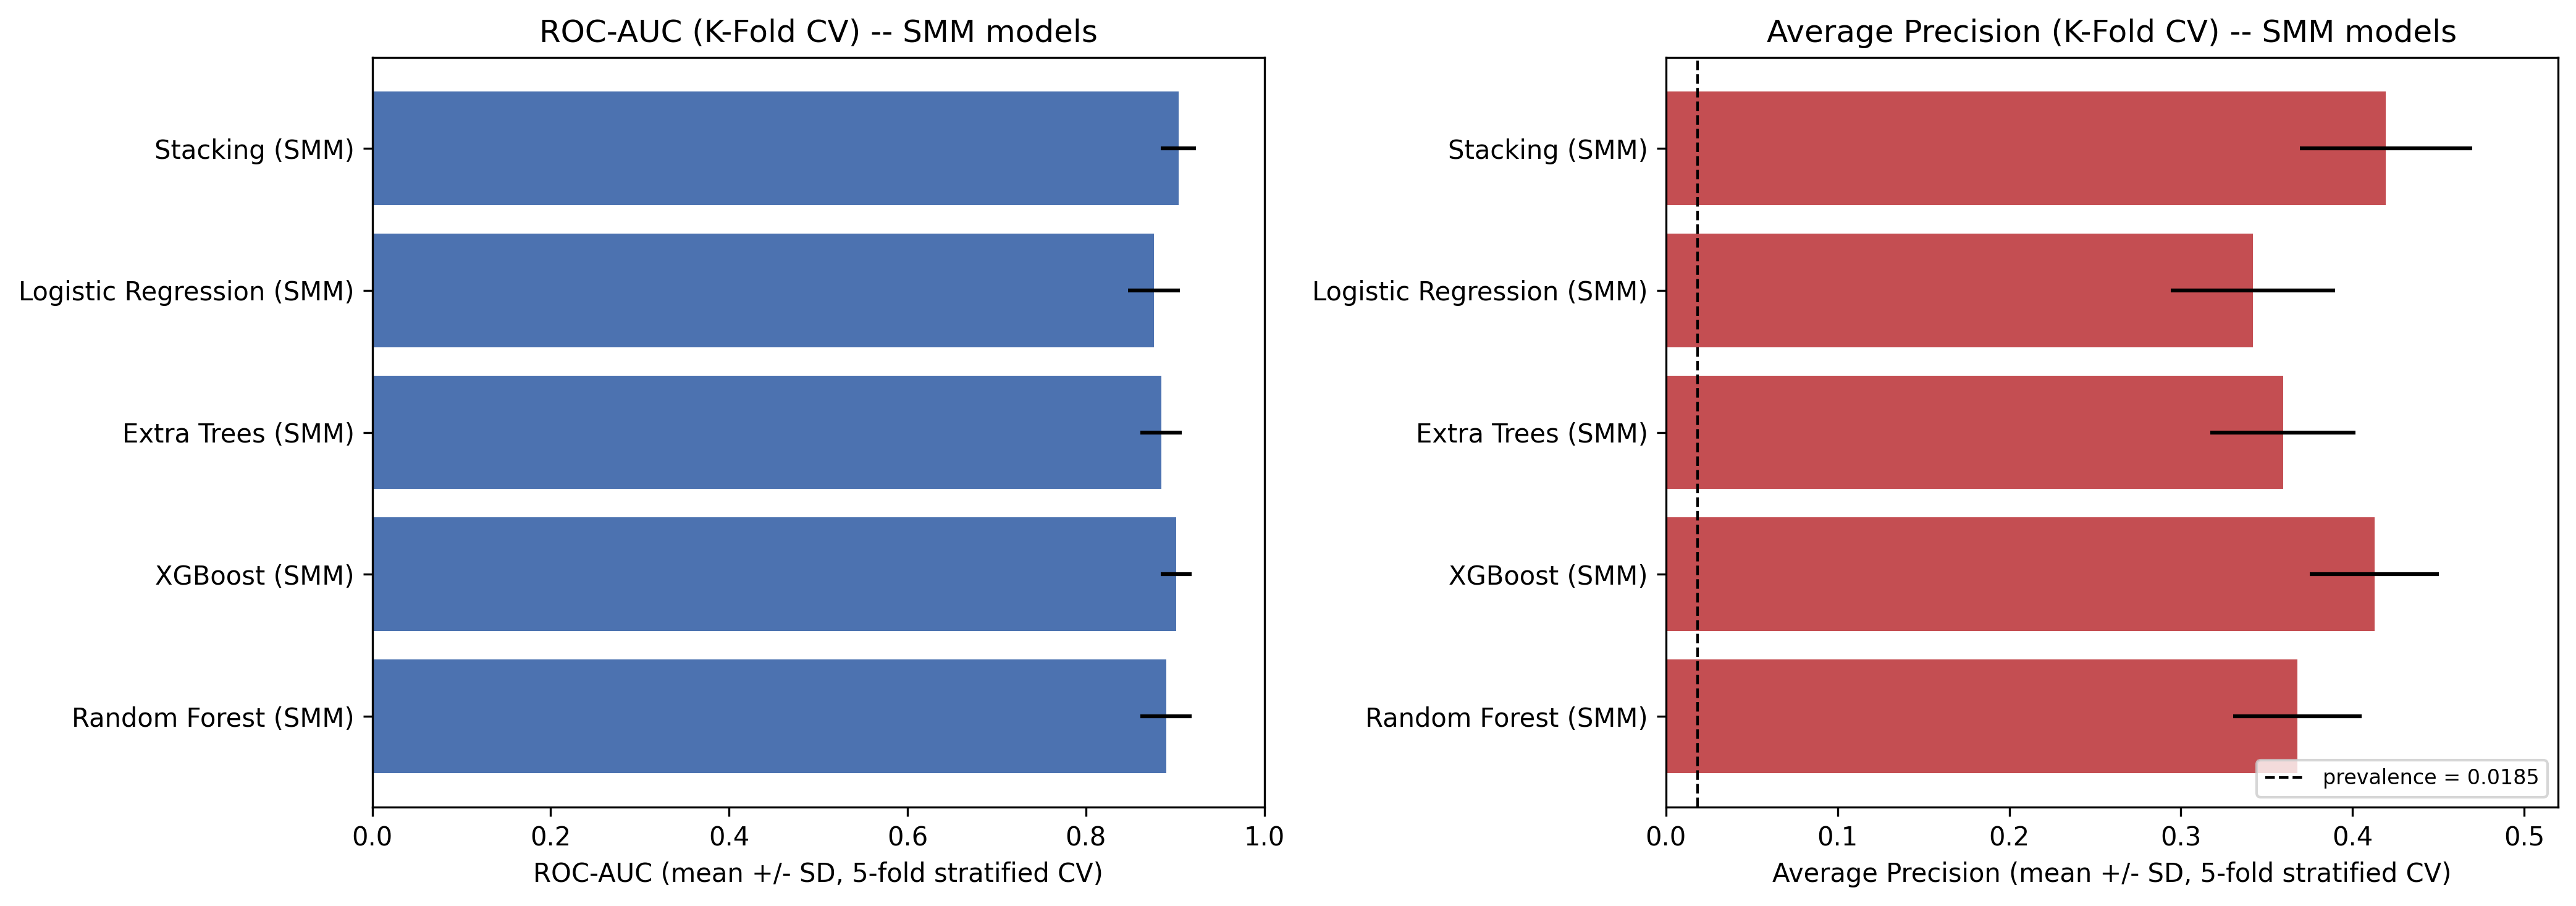
\includegraphics[width=\textwidth]{fig_cv_B.png}
\caption{Model~B: five-fold cross-validated AUC and AP (mean and standard deviation); the dashed line is the prevalence.}\label{fig:cvB}
\end{figure}

\paragraph{Oversampling sensitivity analysis (Model B).}
SMOTE did not improve the precision-based metrics of Model~B either (Table~\ref{tab:smoteB}, Figure~\ref{fig:smoteB}).
The AP of the stacked ensemble went from 0.419 to 0.406 and that of XGBoost from 0.413 to 0.350, while
the AUC of the stacked ensemble went from 0.904 to 0.896. Only Random Forest (AUC 0.890 to 0.899) and LR (AP 0.342 to
0.357) showed small gains. SMOTE shifted the operating point instead: the recall of XGBoost rose from
0.758 to 0.964, but with an F1 of 0.047, that is, almost all admissions were flagged, whereas the recall of the stacked ensemble fell from 0.800 to
0.636. As in Model~A, class weighting was kept as the default.

\begin{table}[H]
\caption{Model~B: effect of SMOTE (sampling strategy 0.2) on five-fold
cross-validated AUC, AP and recall (mean values).\label{tab:smoteB}}
\small
\begin{tabularx}{\textwidth}{lCCCCCC}
\toprule
 & \multicolumn{2}{c}{\textbf{AUC}} & \multicolumn{2}{c}{\textbf{AP}} & \multicolumn{2}{c}{\textbf{Recall}}\\
\cmidrule(lr){2-3}\cmidrule(lr){4-5}\cmidrule(lr){6-7}
\textbf{Model} & Weights & SMOTE & Weights & SMOTE & Weights & SMOTE\\
\midrule
Random Forest & 0.890 & 0.899 & 0.368 & 0.366 & 0.467 & 0.539\\
XGBoost & 0.901 & 0.892 & 0.413 & 0.350 & 0.758 & 0.964\\
Extra Trees & 0.885 & 0.875 & 0.359 & 0.349 & 0.560 & 0.535\\
Logistic Regression & 0.876 & 0.825 & 0.342 & 0.357 & 0.749 & 0.554\\
Stacking & 0.904 & 0.896 & 0.419 & 0.406 & 0.800 & 0.636\\
\bottomrule
\end{tabularx}
\end{table}
\unskip
\begin{figure}[H]
\centering
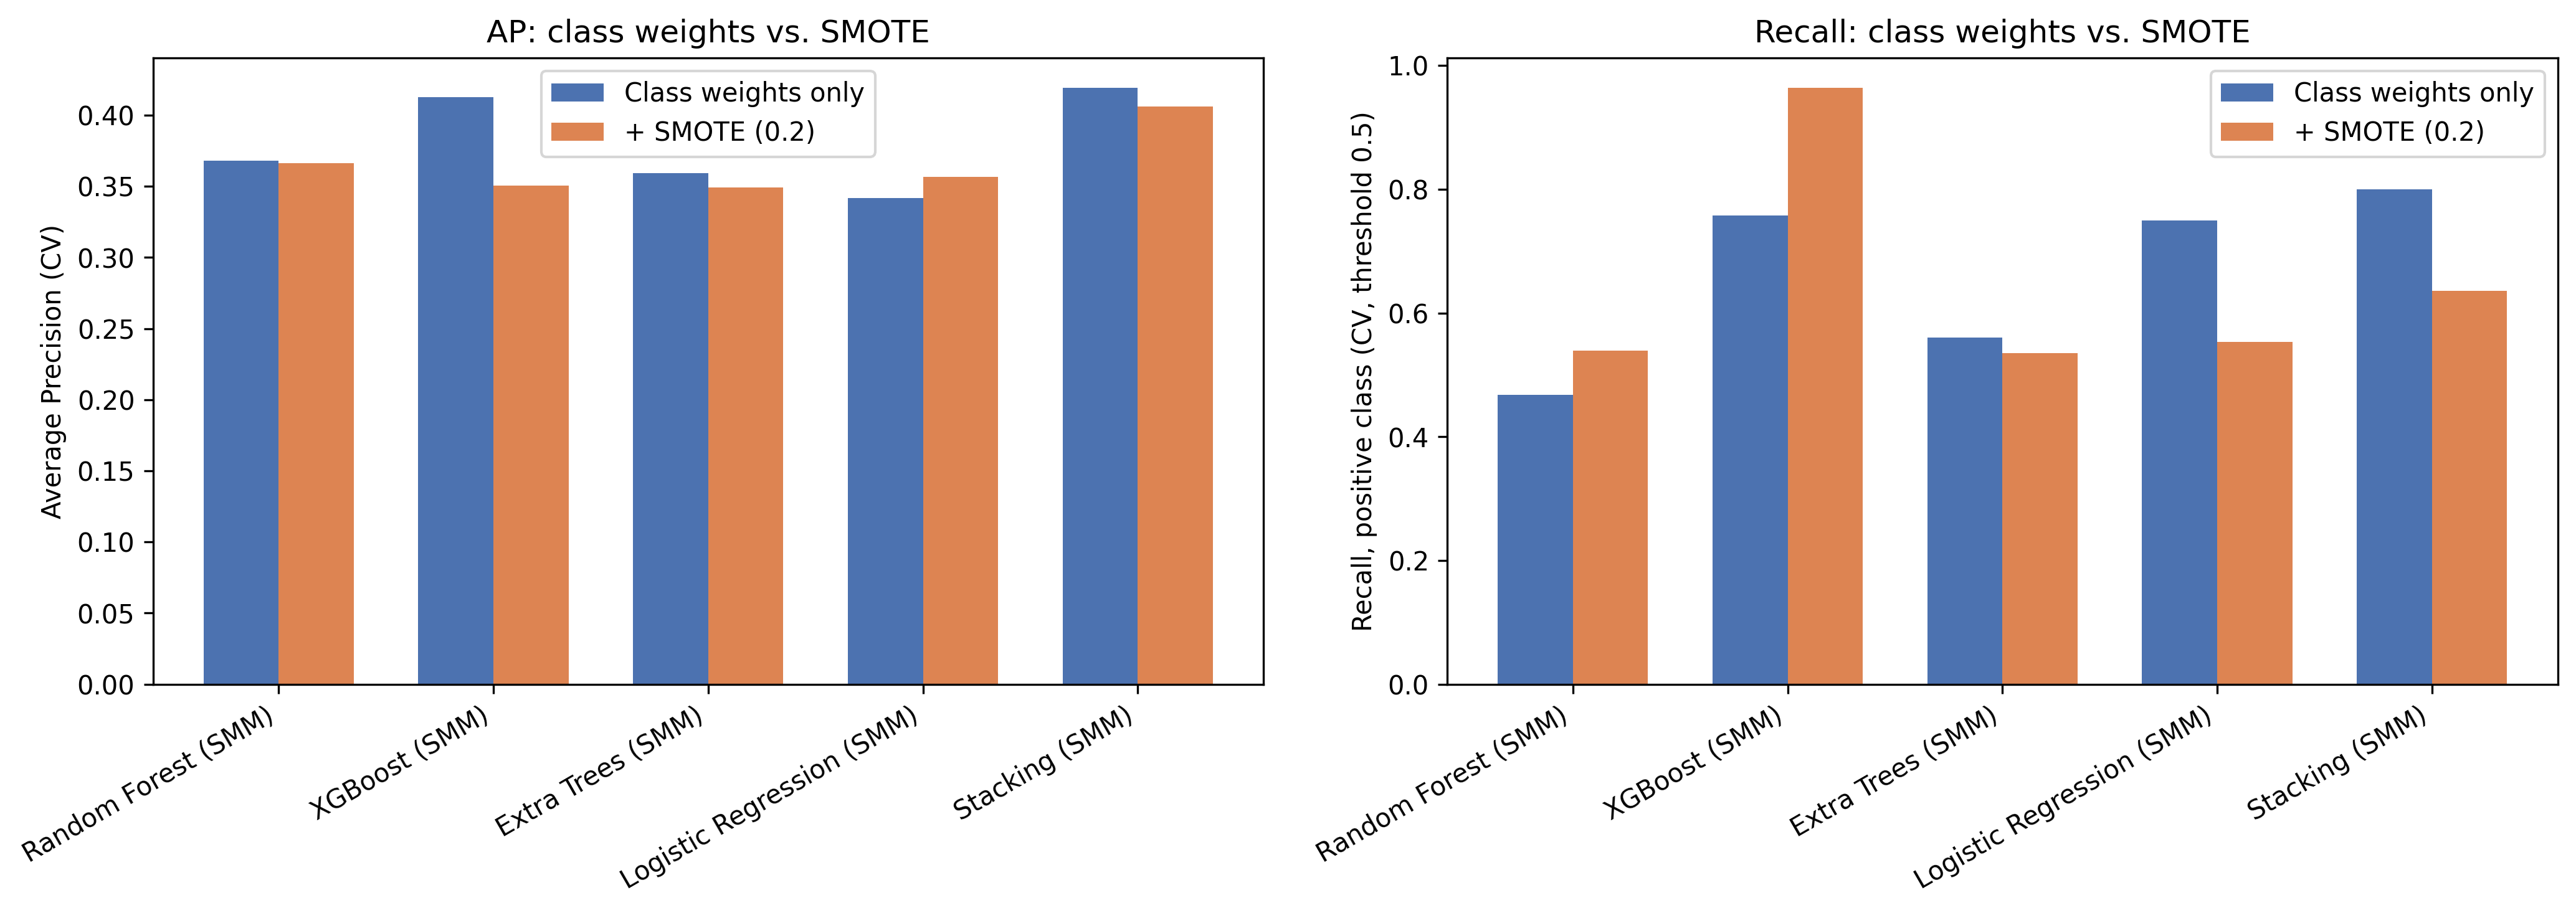
\includegraphics[width=\textwidth]{fig_smote_B.png}
\caption{Model~B: class weighting versus SMOTE in five-fold cross-validation (left: AP; right: recall at threshold 0.5).}\label{fig:smoteB}
\end{figure}

\paragraph{Model A without diagnostic groups.}
Table~\ref{tab:nogdg} compares the cross-validated performance of Model~A with and without the
26 diagnostic-group indicators. Removing them lowered the AUC of every model
(stacking 0.857 to 0.725, RF 0.809 to 0.700, XGB 0.817 to 0.690, ET 0.831 to 0.768, LR 0.758 to
0.635) and brought AP down for four of the five models (to 0.007--0.039; stacking 0.156 to 0.013, against a
prevalence of 0.0016); only LR rose (0.049 to 0.061, with a standard deviation of 0.062). On the hold-out set, the stacked ensemble fell from an AUC of 0.844 and an AP of
0.148 to 0.731 and 0.020 (eight positives; illustrative only). Most of the discriminative signal of Model~A
therefore comes from the diagnosis groups, which are derived from the ICD codes of the admission itself.

\begin{table}[H]
\caption{Model~A: cross-validated AUC and AP with and without the diagnostic-group
indicators (hyperparameters kept; mean values).\label{tab:nogdg}}
\small
\begin{tabularx}{\textwidth}{lCCCC}
\toprule
 & \multicolumn{2}{c}{\textbf{AUC}} & \multicolumn{2}{c}{\textbf{AP}}\\
\cmidrule(lr){2-3}\cmidrule(lr){4-5}
\textbf{Model} & With & Without & With & Without\\
\midrule
Random Forest & 0.809 & 0.700 & 0.115 & 0.007\\
XGBoost & 0.817 & 0.690 & 0.165 & 0.039\\
Extra Trees & 0.831 & 0.768 & 0.190 & 0.021\\
Logistic Regression & 0.758 & 0.635 & 0.049 & 0.061\\
Stacking & 0.857 & 0.725 & 0.156 & 0.013\\
\bottomrule
\end{tabularx}
\end{table}

\paragraph{Calibration and risk stratification of Model A.}
Using the out-of-fold probabilities of the stacked ensemble over the full cohort (41 deaths), the AUC was 0.842
(bootstrap 95\% confidence interval 0.771--0.914) and the AP was 0.123 (0.036--0.251). As expected after
class weighting, the predicted probabilities were far above the observed frequency: the mean predicted
probability was 0.379 against an observed prevalence of 0.0016 (ratio 237.8), the Brier score was 0.162
(0.0016 for a model that always predicts the prevalence; Brier skill score $-100.9$), and the reliability curve lay
below the diagonal over its whole range (Figure~\ref{fig:calibA}). Rank-based measures do not depend on calibration
(Table~\ref{tab:topxA}). Flagging the top 5\% of admissions (1{,}287) captured 18 of the 41 deaths (recall 0.439,
95\% confidence interval 0.286--0.615; positive predictive value 0.014, 0.008--0.021; lift 8.8). With
percentile-based risk bands, the observed mortality was 0.06\% in the low band (below the 80th percentile; 12 deaths
among 20{,}588 admissions), 0.28\% in the moderate band (80th to 95th percentile; 11 of 3{,}861) and 1.40\% in the high band
(top 5\%; 18 of 1{,}287), a roughly 24-fold gradient between the high and the low band. On the hold-out set, 4 of the 8
deaths fell in the high band, 3 in the moderate band and 1 in the low band.

\begin{table}[H]
\caption{Model~A: ``flag the top $x$\%'' table from out-of-fold predictions of the stacked ensemble
(41 deaths among 25{,}736 admissions).\label{tab:topxA}}
\small
\begin{tabularx}{\textwidth}{lCCCCC}
\toprule
\textbf{Top $x$\% flagged} & \textbf{Admissions} & \textbf{Deaths captured} & \textbf{Recall} & \textbf{PPV} & \textbf{Lift}\\
\midrule
0.5\% & 129 & 11 & 0.268 & 0.0853 & 53.5\\
1\% & 257 & 13 & 0.317 & 0.0506 & 31.8\\
2\% & 515 & 14 & 0.341 & 0.0272 & 17.1\\
5\% & 1{,}287 & 18 & 0.439 & 0.0140 & 8.8\\
10\% & 2{,}574 & 22 & 0.537 & 0.0085 & 5.4\\
20\% & 5{,}147 & 29 & 0.707 & 0.0056 & 3.5\\
\bottomrule
\end{tabularx}
\end{table}
\unskip
\begin{figure}[H]
\centering
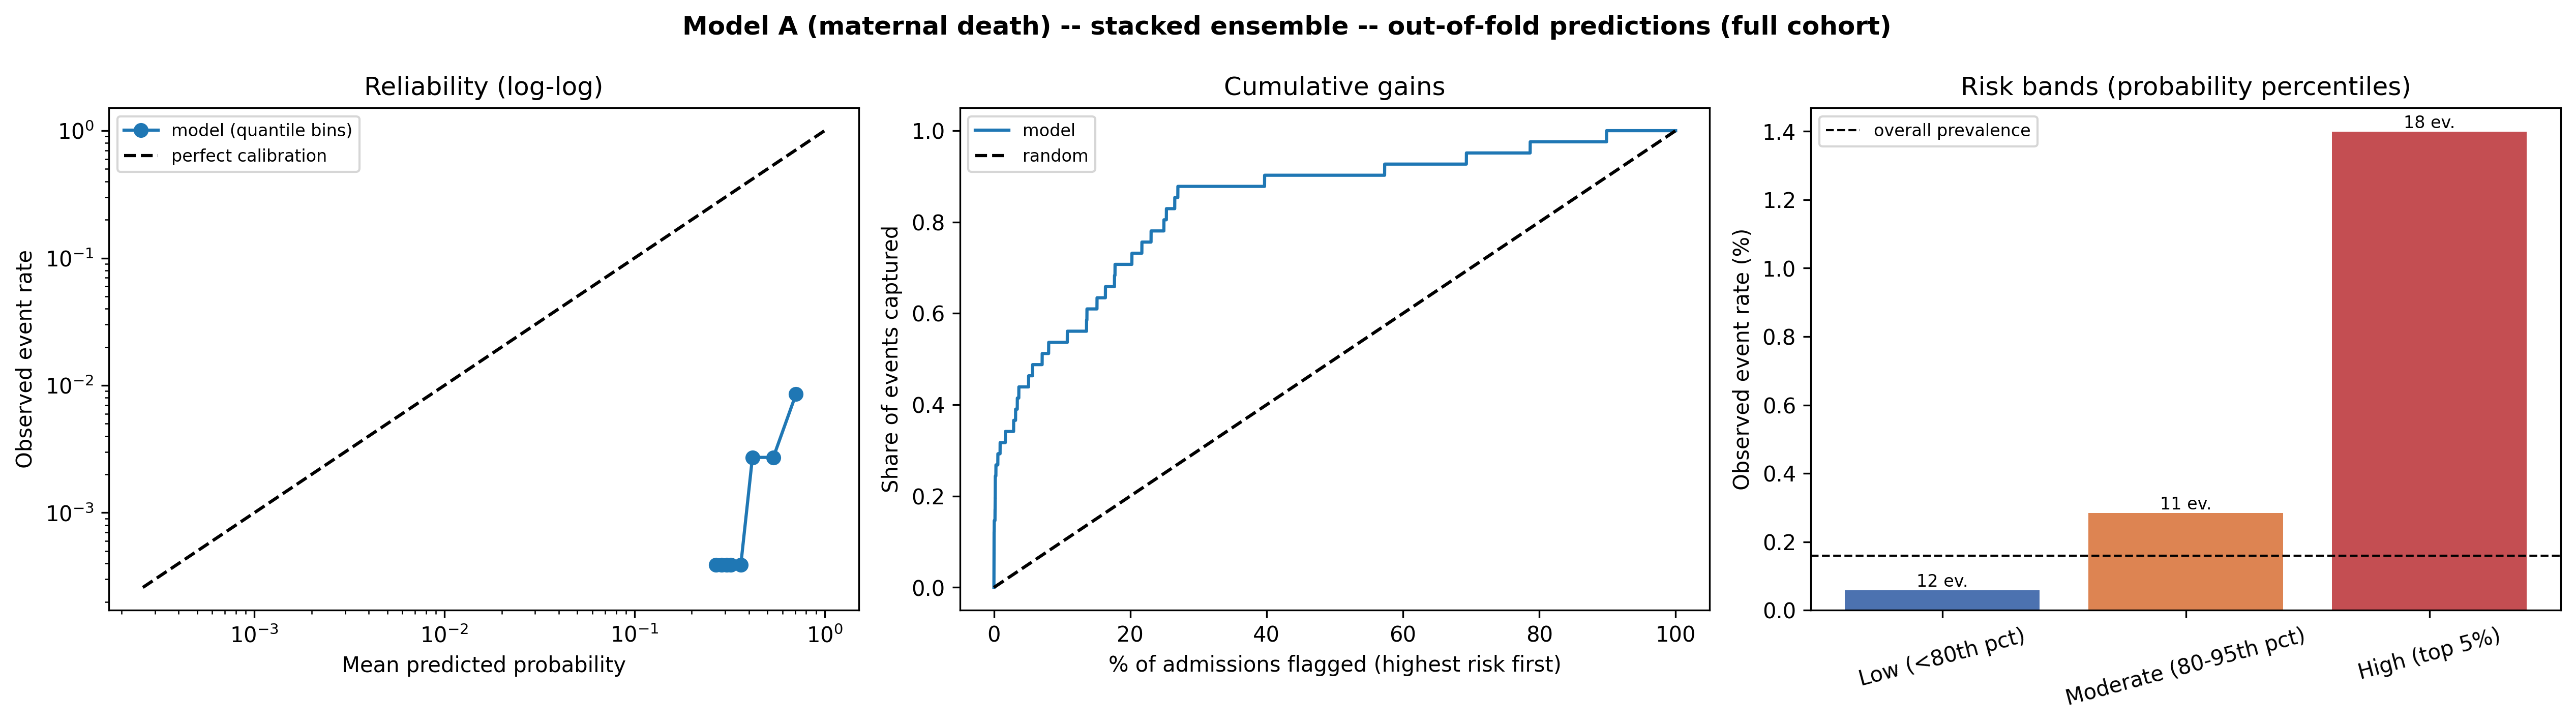
\includegraphics[width=\textwidth]{fig_calib_A_oof.png}
\caption{Model~A, stacked ensemble, out-of-fold predictions over the full cohort: reliability curve (log--log
scale), cumulative gains and observed mortality by risk band.}\label{fig:calibA}
\end{figure}

\paragraph{Calibration and risk stratification of Model B.}
The out-of-fold probabilities of the stacked ensemble over the full cohort (475 SMM cases) gave an AUC of 0.902
(bootstrap 95\% confidence interval 0.884--0.920) and an AP of 0.396 (0.349--0.454). The probabilities were
again much higher than the observed frequency: the mean predicted probability was 0.249 against a prevalence of 0.0185
(ratio 13.5), the Brier score was 0.092 (0.018 for a model that always predicts the prevalence; Brier skill score $-4.10$),
and the reliability curve lay below the diagonal (Figure~\ref{fig:calibB}). The hold-out set showed the same pattern (mean predicted
probability 0.252, ratio 13.6; Brier score 0.093). The raw probabilities should therefore be used to rank admissions and not as absolute risks (see the recalibration below).
In ranking terms (Table~\ref{tab:topxB}), flagging the top 5\% of admissions (1{,}287) captured 324 of the 475 SMM cases
(recall 0.682, bootstrap 95\% confidence interval 0.643--0.719; positive predictive value 0.252, 0.226--0.277; lift 13.6),
and flagging the top 1\% (257) already captured 151 cases with a positive predictive value of 0.588. With percentile-based
risk bands, the observed SMM rate was 0.34\% in the low band (70 cases among 20{,}588 admissions), 2.10\% in the moderate band
(81 of 3{,}861) and 25.2\% in the high band (324 of 1{,}287), a gradient of about 74 times between the high and the low band; the
high band contained 68\% of all cases and the low band 15\%. In the hold-out set, 64 of the 95 cases fell in the high band (observed rate 24.8\%),
19 in the moderate band (2.5\%) and 12 in the low band (0.29\%); recall and positive predictive value in the top 5\% were 0.674 (0.589--0.780) and 0.249 (0.195--0.309).
Percentile-based bands were used because the probability cut-offs (0.27 and 0.80 for the moderate and high bands) are specific to this
model and are not meaningful as absolute risks.

\begin{table}[H]
\caption{Model~B: ``flag the top $x$\%'' table from out-of-fold predictions of the stacked ensemble
(475 SMM cases among 25{,}736 admissions).\label{tab:topxB}}
\small
\begin{tabularx}{\textwidth}{lCCCCC}
\toprule
\textbf{Top $x$\% flagged} & \textbf{Admissions} & \textbf{Cases captured} & \textbf{Recall} & \textbf{PPV} & \textbf{Lift}\\
\midrule
0.5\% & 129 & 79 & 0.166 & 0.612 & 33.2\\
1\% & 257 & 151 & 0.318 & 0.588 & 31.8\\
2\% & 515 & 238 & 0.501 & 0.462 & 25.0\\
5\% & 1{,}287 & 324 & 0.682 & 0.252 & 13.6\\
10\% & 2{,}574 & 372 & 0.783 & 0.145 & 7.8\\
20\% & 5{,}147 & 405 & 0.853 & 0.079 & 4.3\\
\bottomrule
\end{tabularx}
\end{table}
\unskip
\begin{figure}[H]
\centering
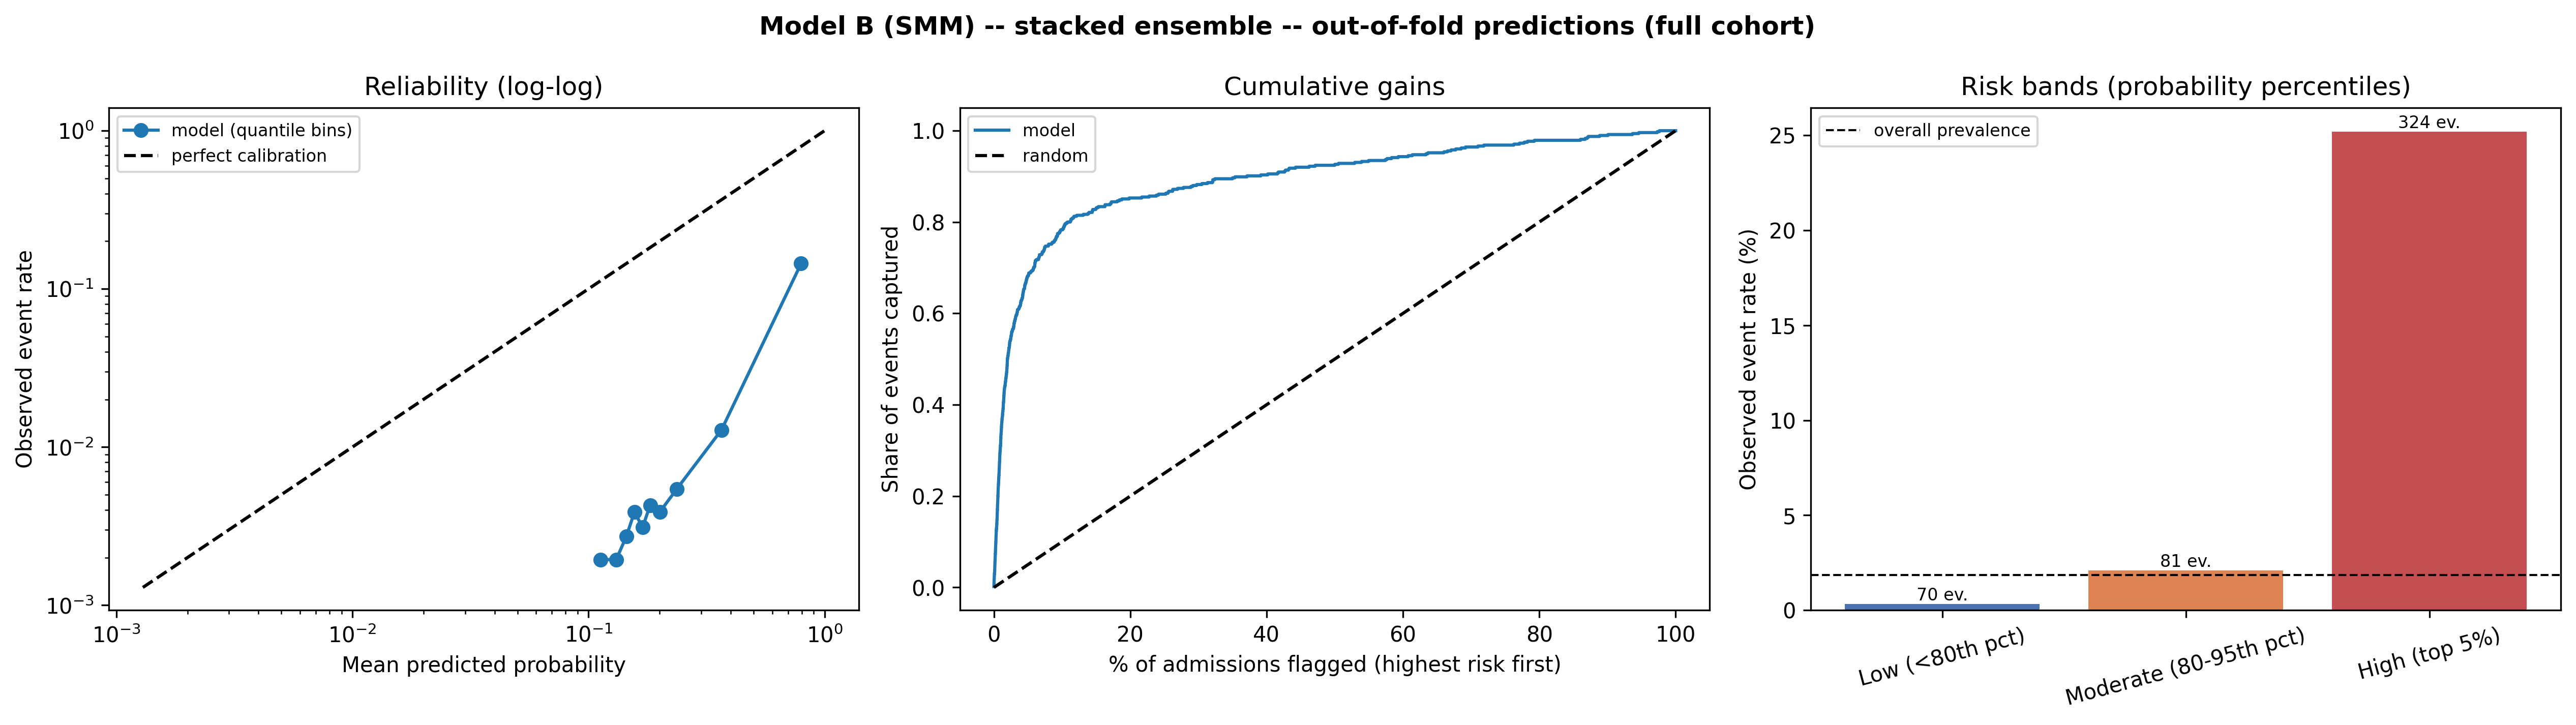
\includegraphics[width=\textwidth]{fig_calib_B_oof.png}
\caption{Model~B, stacked ensemble, out-of-fold predictions over the full cohort: reliability curve (log--log
scale), cumulative gains and observed SMM rate by risk band.}\label{fig:calibB}
\end{figure}

\paragraph{Recalibration.}
Because class weighting inflates the predicted probabilities, we recalibrated the out-of-fold probabilities of the stacked
ensemble post hoc (Table~\ref{tab:recal}, Figure~\ref{fig:recal}). For Model~B, Platt scaling brought the ratio of mean predicted probability
to prevalence from 13.5 to 1.00, reduced the ECE from 0.231 to 0.0009, set the calibration slope to 1.00 and turned the Brier skill score from
$-4.10$ to 0.26 (Brier score 0.0134 against 0.0925), with practically unchanged discrimination (AUC 0.902 to 0.901; AP 0.396 to 0.394).
Isotonic regression gave similar calibration (Brier skill score 0.256) but slightly lower discrimination (AUC 0.895; AP 0.370), as expected from a
step function that creates ties between probabilities. For Model~A, Platt scaling also removed most of the miscalibration (ratio 237.8 to 1.01; ECE 0.377 to 0.0006), but the Brier
skill score reached only 0.064, because the Brier score (0.0015) is barely below that of a model that always predicts the prevalence (0.0016), and the AUC fell from 0.842 to 0.836
(AP 0.123 to 0.115). Isotonic regression was less stable for Model~A (calibration slope 0.73; AUC 0.805; AP 0.098), as 41 events do not support a flexible calibration map.
Recalibration therefore turns the scores of Model~B into usable risk estimates in this cohort, whereas for Model~A it makes them calibrated
but hardly more informative than the prevalence. The calibration maps were estimated by repeated cross-validation within the same cohort and
still require external validation.

\begin{table}[H]
\caption{Post hoc recalibration of the out-of-fold stacking probabilities (mean of 20 repetitions of five-fold cross-validation): Brier score and
Brier skill score (relative to a model that predicts the prevalence), ratio of mean predicted probability to prevalence, expected calibration error (ECE, ten quantile bins),
calibration slope, AUC and AP.\label{tab:recal}}
\scriptsize
\setlength{\tabcolsep}{3pt}
\begin{tabularx}{\textwidth}{llCCCCCCC}
\toprule
\textbf{Model} & \textbf{Probabilities} & \textbf{Brier} & \textbf{Skill} & \textbf{Ratio} & \textbf{ECE} & \textbf{Slope} & \textbf{AUC} & \textbf{AP}\\
\midrule
A (mortality) & Raw (class-weighted) & 0.1621 & $-100.9$ & 237.8 & 0.377 & 1.08 & 0.842 & 0.123\\
 & Platt & 0.0015 & 0.064 & 1.01 & 0.0006 & 0.98 & 0.836 & 0.115\\
 & Isotonic & 0.0015 & 0.055 & 1.01 & 0.0006 & 0.73 & 0.805 & 0.098\\
\midrule
B (SMM) & Raw (class-weighted) & 0.0925 & $-4.10$ & 13.5 & 0.231 & 1.04 & 0.902 & 0.396\\
 & Platt & 0.0134 & 0.260 & 1.00 & 0.0009 & 1.00 & 0.901 & 0.394\\
 & Isotonic & 0.0135 & 0.256 & 1.00 & 0.0011 & 0.97 & 0.895 & 0.370\\
\bottomrule
\end{tabularx}
\end{table}
\unskip
\begin{figure}[H]
\centering
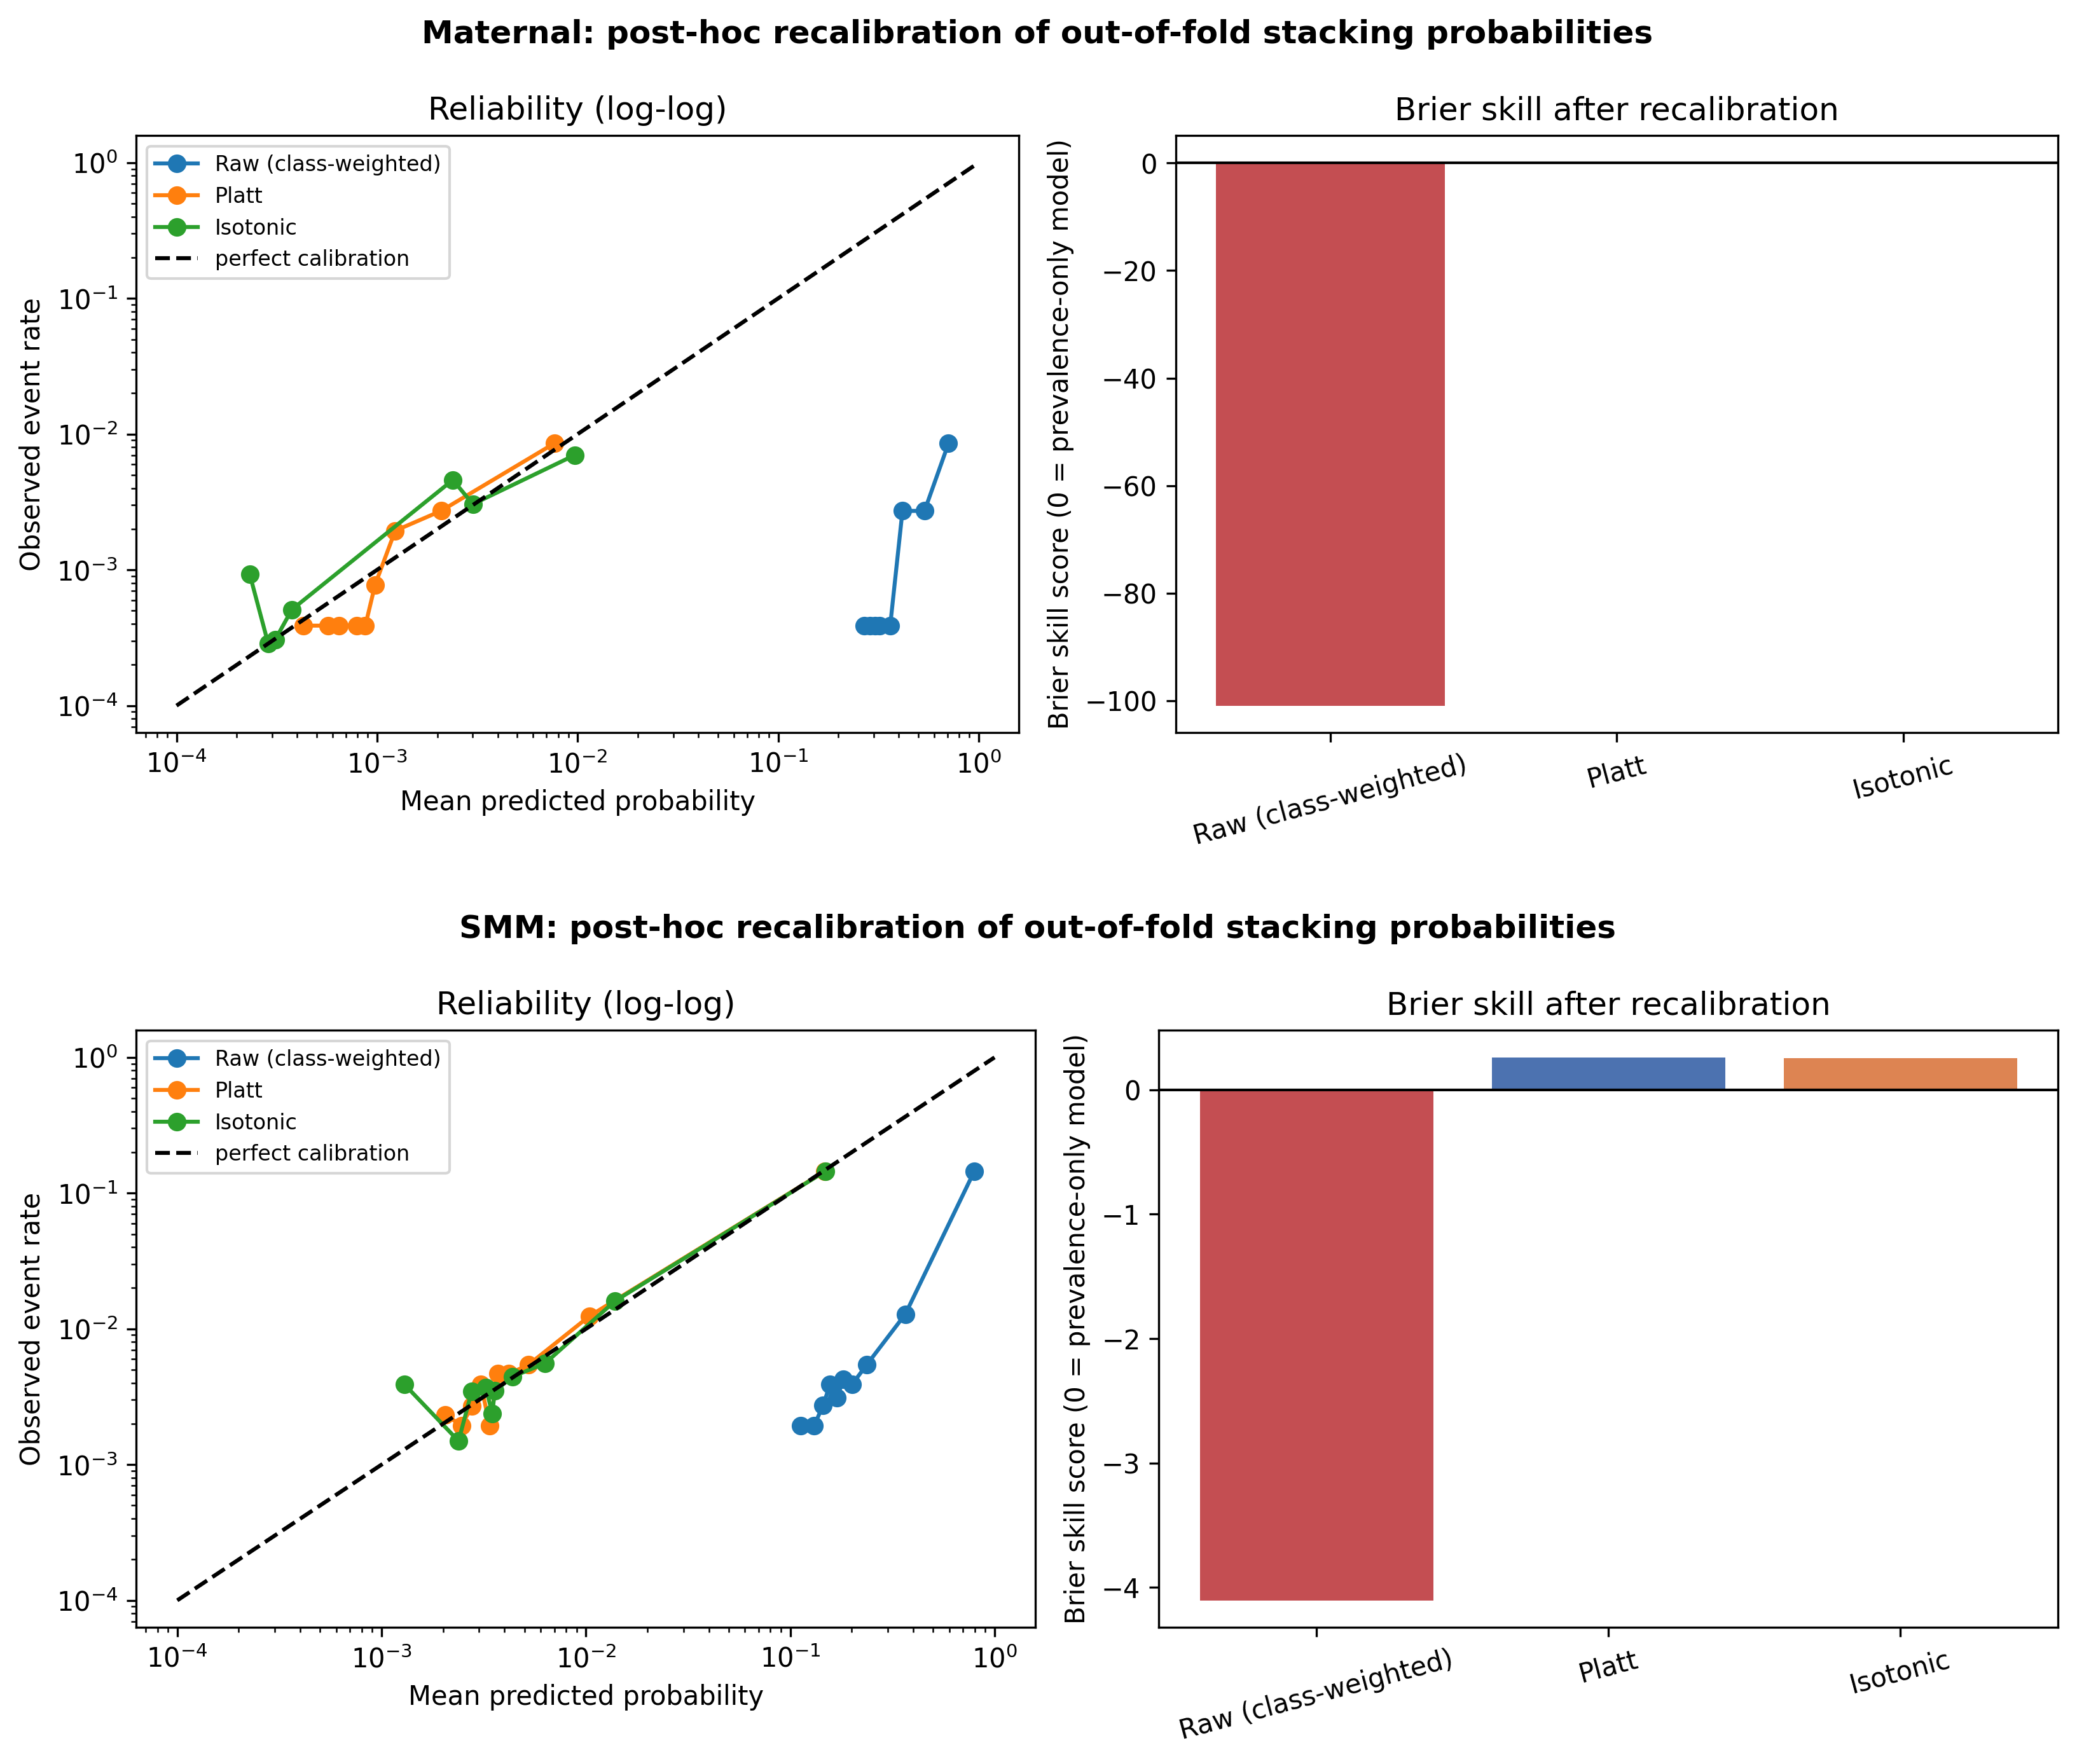
\includegraphics[width=0.85\textwidth]{fig_recal.png}
\caption{Post hoc recalibration of the out-of-fold stacking probabilities: reliability curves (log--log scale) and Brier skill score
for Model~A (top) and Model~B (bottom).}\label{fig:recal}
\end{figure}

\paragraph{Explainability and subgroup audit.}
The mean absolute SHAP values of the XGBoost base learner on the test set were highest for creatinine (0.28),
glucose (0.24), ICU stay (0.24), bicarbonate (0.18), lactic acid (0.16), magnesium (0.14), age (0.13) and
hemoglobin (0.13), followed by hematocrit, observation and urgent admission types, and transfer admissions (0.08--0.09)
(Figure~\ref{fig:shap}). The ranking agrees with the Random Forest importances (renal and metabolic laboratory values at the top) and adds ICU stay and
lactic acid. These are descriptions of the fitted model and not causal effects; moreover, ICU stay and lactate may follow
the morbid event rather than precede it, so their weight should be read with the timing caveat discussed below.

\begin{figure}[H]
\centering
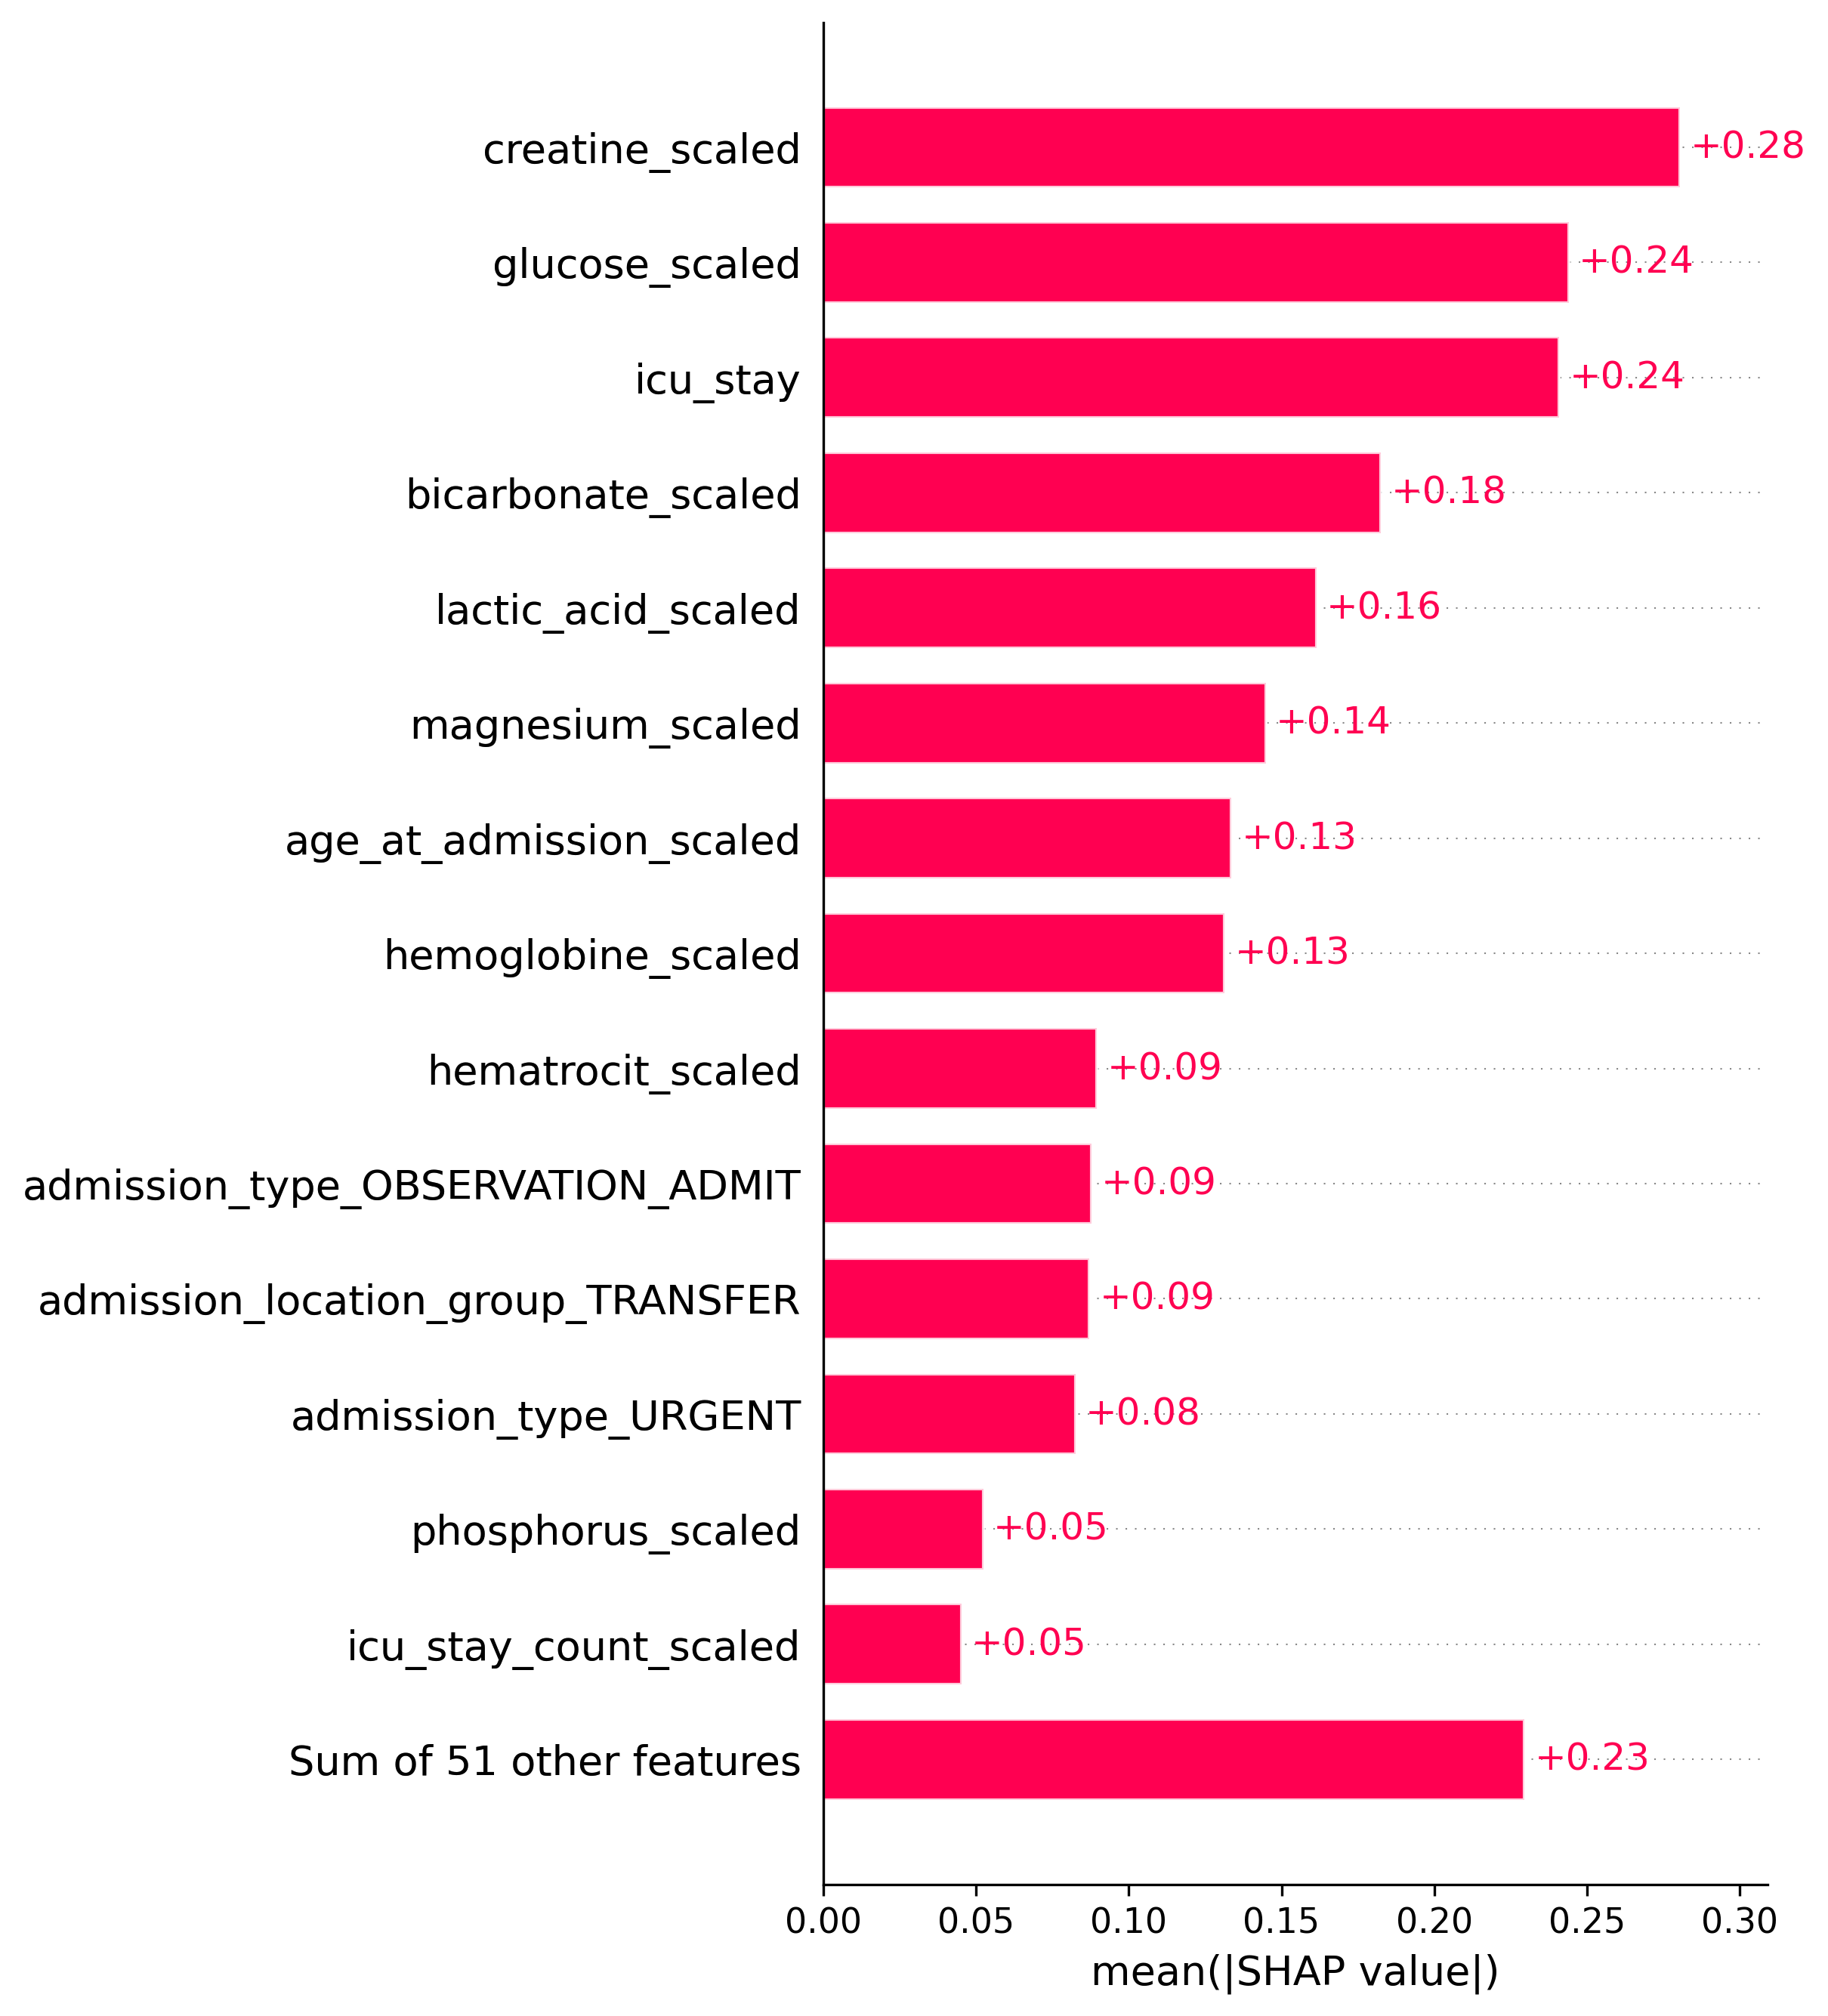
\includegraphics[width=0.6\textwidth]{fig_shap_bar_B.png}
\caption{Model~B: mean absolute SHAP value of the 15 most influential predictors of the XGBoost base learner (test set).
Variable names are those of the notebook; the suffix \texttt{\_scaled} denotes the scaled version of each variable.}\label{fig:shap}
\end{figure}

On the hold-out set, the AUC of the stacked ensemble was between 0.86 and 0.95 in nearly all subgroups with at least 10 positive
admissions (Table~\ref{tab:subgroup}); the confidence intervals were wide and overlapped for ethnicity groups, insurance
categories and age quartiles, so no difference between them can be asserted. Subgroups with fewer than 10 positives (Asian,
Hispanic, Indian-American, European-White and Pacific-Islander groups; Medicare, other insurance and unclassified insurance) were not evaluated. The clear exception
was the 94 admissions with an ICU stay, among which 36 (38\%) were SMM cases and the AUC was 0.655 (0.539--0.767): the model flagged
99\% of them, so ICU stay was a strong predictor of SMM by itself but the model did not separate cases from
non-cases inside this group. Performance was similar in delivery (AUC 0.920) and non-delivery hospitalizations (0.913), although the AP was three
times higher in the former (0.646 against 0.221), reflecting its higher prevalence. All subgroup estimates are descriptive, are based on a single test split, and do not
constitute a formal fairness assessment.

\begin{table}[H]
\caption{Model~B: hold-out performance of the stacked ensemble by subgroup. Only subgroups with at least 10 positive admissions are shown.
Age groups correspond to the quartiles of the scaled age, approximately $\leq$28, 29--32, 33--36 and $\geq$37 years.\label{tab:subgroup}}
\small
\begin{tabularx}{\textwidth}{llccCc}
\toprule
\textbf{Dimension} & \textbf{Subgroup} & \textbf{Admissions} & \textbf{SMM cases} & \textbf{AUC (95\% CI)} & \textbf{AP}\\
\midrule
Ethnicity group & AFRO\_DESC & 1{,}285 & 28 & 0.866 (0.769--0.946) & 0.304\\
 & UNKNOWN & 619 & 17 & 0.944 (0.865--0.984) & 0.532\\
 & WHITE\_USA & 2{,}092 & 39 & 0.921 (0.868--0.965) & 0.355\\
Insurance & Medicaid & 1{,}731 & 32 & 0.902 (0.820--0.967) & 0.430\\
 & Private & 3{,}194 & 60 & 0.923 (0.878--0.963) & 0.405\\
Age & $\leq$28 years & 1{,}312 & 20 & 0.884 (0.773--0.968) & 0.351\\
 & 29--32 years & 1{,}271 & 18 & 0.940 (0.862--0.986) & 0.317\\
 & 33--36 years & 1{,}333 & 29 & 0.953 (0.917--0.982) & 0.473\\
 & $\geq$37 years & 1{,}232 & 28 & 0.860 (0.763--0.949) & 0.404\\
ICU stay & Yes & 94 & 36 & 0.655 (0.539--0.767) & 0.609\\
 & No & 5{,}054 & 59 & 0.873 (0.815--0.929) & 0.219\\
Hospitalization & Delivery & 1{,}802 & 58 & 0.920 (0.874--0.963) & 0.646\\
 & Non-delivery & 3{,}346 & 37 & 0.913 (0.851--0.960) & 0.221\\
\bottomrule
\end{tabularx}
\end{table}

%--------------------------------------------------------------------
\section{Discussion}\label{sec:discussion}
%--------------------------------------------------------------------
\textbf{Mortality is not a modelling target at this sample size.} With 41 deaths,
cross-validated AUC values of 0.76--0.86 coexisted with AP of 0.05--0.19, with
standard deviations of AP of the same order as the means, and with hold-out conclusions
supported by eight deaths. A ranking of the five algorithms is therefore not
reliable: for example, LR ranked second in hold-out AUC (0.854) but had the lowest hold-out AP (0.031) and the lowest
cross-validated AUC and AP (0.758 and 0.049), whereas XGB had the highest hold-out AP (0.278)
but a cross-validated AP (0.165) below that of ET (0.190). Our results
support the recommendation to report precision--recall metrics and
fold-level dispersion for rare outcomes~\cite{Marshall2023Imbalance,Saito2015PR}.

\textbf{SMM is a more stable surrogate, but a noisy one.} A positive class eleven
times larger produced hold-out AUC values of 0.889--0.913 with a narrow spread across
algorithms, a stacked ensemble that was best on both AUC and AP on the hold-out set and in cross-validation
(0.904 $\pm$ 0.020 and 0.419 $\pm$ 0.050, with fold-to-fold standard deviations of the AUC about one
third of those of Model~A), and a precision--recall trade-off that can be discussed clinically.
In ranking terms, the top 5\% of admissions held 68\% of SMM cases with a positive predictive value of 0.25
(lift 13.6). Two limitations
should be stated plainly. First, the SMM label is ICD-based; ICD-10 coding showed
low sensitivity and positive predictive value in a medical-record validation
study~\cite{Boulet2024ICD10SMM}, so our positives are an administrative proxy, and
the model may partly learn coding and care-intensity patterns. This is also likely
to explain the high SMM rate in delivery hospitalizations. Second, the leading
predictors of Model~B were creatinine, glucose, bicarbonate and magnesium,
which relate to renal and metabolic derangement; since acute renal failure is the
most frequent indicator (180 admissions), part of the signal reflects
laboratory abnormalities that co-occur with the outcome definition rather than
anticipate it. Using the earliest available value mitigates but does not remove this
concern, and prospective timing of predictors relative to the event was not
enforced. The SHAP analysis and the subgroup audit point in the same direction: ICU stay and lactic acid
ranked among the most influential predictors, and the AUC was lowest (0.655) in the 94 test admissions with an ICU stay, where
36 were SMM cases and the model flagged 99\%; ICU stay is therefore itself a strong marker of SMM, but the model does not
separate cases from non-cases among the critically ill. Differences across ethnicity, insurance and age groups were not distinguishable from sampling noise
(overlapping intervals based on 17--60 positives per subgroup), and no claim about equity can be made from them.

\textbf{Oversampling and outlier policy.} SMOTE did not improve the precision-based
metrics in either model (stacking AP 0.156 to 0.168 in Model~A and 0.419 to 0.406 in Model~B), and it shifted the
operating point in unpredictable ways (XGBoost recall in Model~B 0.758 to 0.964 with an F1 of 0.047), in line with evidence that imbalance corrections can harm calibration
and do not necessarily improve discrimination~\cite{vandenGoorbergh2022Harm}.
Replacing row deletion by winsorization preserved all positive cases;
retaining them matters more than the geometric tidiness of the feature
distribution, since deleting extreme laboratory values removes precisely the
sickest patients.

\textbf{Limitations.} (i) Single-center data and no external validation. (ii)
Model~A includes the 26 diagnosis-group indicators whereas Model~B excludes them; the
two models are therefore not strictly comparable in predictor sets. Removing the indicators from
Model~A lowered its cross-validated AUC from 0.857 to 0.725 and its AP from 0.156 to 0.013, so its
performance with the groups depends on variables derived from the admission's own diagnoses, which may
reflect the clinical course leading to death rather than anticipate it. (iii) Imputation values and scalers
were fitted before the train/test split, and the cross-validation re-fits
hyperparameters tuned on the training split, which can make estimates slightly
optimistic. (iv) The ICD-based SMM label and the laboratory and ICU-related predictors may be partly concurrent with the
event (the timing of predictors relative to the event was not enforced). (v) The mortality
outcome captures only deaths recorded by the hospital; post-discharge deaths are not
observed. (vi) Metrics at the default 0.5 threshold are shown for transparency;
raw probabilities were 13.5 times (Model~B) and 238 times (Model~A) higher than the observed
prevalence because of class weighting~\cite{NiculescuMizil2005Probabilities,vandenGoorbergh2022Harm,VanCalster2019Calibration}; post hoc recalibration corrected them, but the calibration maps were
estimated in the same cohort by repeated cross-validation and have not been validated externally, isotonic regression was unstable for Model~A with 41 events,
and no threshold optimization was carried out. (vii) MIMIC-IV is not an obstetric
registry and may differ from the population of obstetric services in
other health systems. The models are research prototypes and should not guide
individual clinical decisions.

%--------------------------------------------------------------------
\section{Implications and Future Work}\label{sec:implications}
%--------------------------------------------------------------------
\textbf{Implications for practice.} The results do not support using either model for
individual decisions. They do indicate how a maternal risk tool should be designed:
as a ranking of admissions for review rather than a classifier at a default threshold,
with the share of admissions flagged chosen by a clinical panel in view of the recall
and precision trade-off, and with absolute risks recalibrated before display. Any
operating point or action triggered by such a tool in obstetric care requires validation
by an authorized human decision-maker.

\textbf{Surveillance rather than prediction.} Because the SMM categories are
clinically distinct (renal, hemorrhagic, respiratory and others), and almost a quarter
of SMM admissions involve more than one category, a hospital could use the same
features to monitor SMM burden by category and to review cases, even if individual
prediction remains imperfect.

\textbf{Ethical considerations and governance.} Four issues deserve explicit mention. First, the data come from a single
academic medical center in the United States and were accessed under the PhysioNet credentialed data use agreement, which prohibits
re-identification and the sharing of raw data with non-credentialed parties; any reuse of these models with other patient
data requires its own authorization and ethical review. Second, regarding algorithmic bias, the subgroup audit
(Table~\ref{tab:subgroup}) was descriptive and could not evaluate several ethnicity and insurance groups for lack of events; the lowest AUCs were
observed in the AFRO\_DESC group (0.866) and, above all, among admissions with an ICU stay (0.655), and predictions may be least
reliable for the groups that are already under-represented in the training data~\cite{Obermeyer2019Bias,Rajkomar2018Fairness}.
Third, regarding transparency, SHAP values describe associations learned by the model and not causal mechanisms, and a leading
predictor may be a proxy for an unmeasured factor; a model card documenting the intended use, the data, the performance by subgroup and the known
limitations~\cite{Mitchell2019ModelCards} would be a minimum requirement for any release of these models. Fourth, regarding human oversight,
the models are research prototypes and should not be used in clinical care; any future tool would have to act as a non-binding
aid whose alerts clinicians can override and document, be preceded by prospective validation and regulatory review in the applicable
jurisdiction, and be monitored after deployment for drift in discrimination and calibration (for example with a rolling AUC and Brier score) overall and by subgroup.

\textbf{Future work.} Five directions follow from the limitations. (i)~External validation
on other hospital cohorts, in particular obstetric services, to test whether the
laboratory-driven signal generalizes; where patient-level data cannot be pooled, federated learning could allow
multicenter training and validation without sharing records~\cite{Rieke2020Federated,Dayan2021Federated}. (ii)~Validation of the ICD-based SMM label against
medical-record review in a sample, to estimate its real sensitivity and positive predictive
value in this cohort. (iii)~Restricting predictors to values recorded before the event, which would turn the SMM
model into a genuine early-warning model. (iv)~External validation of the recalibration maps and decision-curve analysis~\cite{Vickers2006DCA}. (v)~A secondary multiclass model that predicts the primary SMM category
among positive admissions, which answers the clinically distinct question of which complication
is most likely once SMM occurs.

%--------------------------------------------------------------------
\section{Conclusions}\label{sec:conclusions}
%--------------------------------------------------------------------
In 25{,}736 obstetric admissions of MIMIC-IV, in-hospital-recorded maternal death
(41 events) could not be modelled with reliable precision, whereas SMM (475 events)
allowed a stable evaluation, with a stacked ensemble reaching a hold-out AUC of
0.913 and AP of 0.384, confirmed by cross-validation (0.904 and 0.419); the top 5\% of admissions
by predicted probability contained 68\% of SMM cases. The apparent discrimination for mortality depended largely on diagnosis-group
indicators, the raw probabilities of both models were not calibrated (Platt scaling corrected them), and the performance was lowest among admissions with an ICU stay. Class weighting
was preferable to SMOTE, and winsorization protected positive cases from deletion. Future work should validate these models,
including their recalibration, on independent cohorts and define thresholds for a decision-support use
case, and evaluate the secondary multiclass task of predicting the SMM category.

\vspace{6pt}
\authorcontributions{Conceptualization, E.G.J. and J.D.M.D.;
methodology, E.G.J.; software, E.G.J.; validation, E.G.J.;
formal analysis, E.G.J.; investigation, E.G.J.; data curation, E.G.J.;
writing---original draft preparation, E.G.J.;
writing---review and editing, E.G.J. and J.D.M.D.; visualization, E.G.J.;
supervision, J.D.M.D.; funding acquisition, E.G.J. All authors have read and agreed to the published
version of the manuscript.}

\funding{This research was supported by the Becas de Excelencia Doctoral
del Bicentenario program, funded by the Fondo de Ciencia, Tecnolog\'ia
e Innovaci\'on del Sistema General de Regal\'ias (FCTeI-SGR) and
administered by the Ministerio de Ciencia, Tecnolog\'ia e Innovaci\'on (Minciencias) of Colombia.
This support was provided through BPIN~2020000100287, through Universidad
del Norte, Barranquilla, Colombia, as executing institution.}

\institutionalreview{Ethical review and approval were waived for this
study owing to the retrospective, fully de-identified, secondary-use
nature of the MIMIC-IV database. The original collection and
de-identification of the data were reviewed and approved by the
Institutional Review Board of the Beth Israel Deaconess Medical Center
(BIDMC), which granted a waiver of informed consent for the creation and
sharing of the database~\cite{Johnson2023MIMICIV}.}

\informedconsent{Patient consent was waived by the Institutional Review
Board of the Beth Israel Deaconess Medical Center for the original
collection of the MIMIC-IV database, owing to its retrospective and
fully de-identified nature~\cite{Johnson2023MIMICIV}. No participants were
directly recruited by the authors.}

\dataavailability{The clinical data used in this study are available
from the MIMIC-IV database but restrictions apply to their availability:
they were used under a data use agreement and are therefore not publicly
redistributable. Data are available via PhysioNet~\cite{Goldberger2000PhysioNet}
to any researcher who completes the required training and signs the PhysioNet
Credentialed Health Data Use Agreement
(\url{https://physionet.org/content/mimiciv/}). The SQL scripts and notebooks
for cohort extraction, preprocessing and modelling are available at
\url{https://github.com/khem777/maternal-smm-mimicIV}.}

\acknowledgments{The authors thank the MIMIC-IV team at the Laboratory
for Computational Physiology (MIT) and Beth Israel Deaconess Medical
Center for maintaining and providing open access to the database.
The authors also thank the four clinical experts who, voluntarily and without financial compensation, took part in the grouping of diagnosis codes and who asked to remain anonymous.}

\conflictsofinterest{The authors declare no conflicts of interest. The funders had no role in the design of the study; in the collection, analyses, or interpretation of data; in the writing of the manuscript; or in the decision to publish the results.}

\abbreviations{Abbreviations}{
\noindent
\begin{tabular}{@{}ll}
AP    & Average Precision \\
AUC   & Area Under the Receiver Operating Characteristic Curve \\
BIDMC & Beth Israel Deaconess Medical Center \\
CDC   & Centers for Disease Control and Prevention \\
CV    & Cross-Validation \\
ET    & Extra Trees \\
FAD   & Federally Available Data \\
HRSA  & Health Resources and Services Administration \\
ICD   & International Classification of Diseases \\
ICU   & Intensive Care Unit \\
IQR   & Interquartile Range \\
LR    & Logistic Regression \\
MIMIC & Medical Information Mart for Intensive Care \\
ML    & Machine Learning \\
PR    & Precision--Recall \\
RF    & Random Forest \\
ROC   & Receiver Operating Characteristic \\
SMM   & Severe Maternal Morbidity \\
SMOTE & Synthetic Minority Over-sampling Technique \\
XGB   & XGBoost (Extreme Gradient Boosting) \\
\end{tabular}}

\begin{adjustwidth}{-\extralength}{0cm}
\reftitle{References}
\bibliography{bib/bibliography_maternal}
\end{adjustwidth}

\end{document}
